
\section{Introduction}
\emph{Anomaly}, from grec $\alpha\nu\omega\mu\alpha\lambda\iota\alpha$, asperity, irregular, not the same (an-homalos), refers to a gap, a deviation with respect to some norm or basis, reflecting the expected behavior.
We call \emph{anomaly} the underlying object inducing a gap, the observation which deviates from normality. 
%
In various fields, the following situation occurs: an expert aims at predicting a phenomenon based on previous observations. The most basic case is when one wants to predict some binary characteristic of some new observations/records, given previous ones. For instance one can think of a doctor aiming to predict if an incoming patient has a cancer or not, using previous patient record (age, history, gender, blood pressure) associated with their true \textbf{label} (having cancer or not). This case is an example of \emph{binary classification}: the doctor aims to find a rule to \textbf{predict} the label of a new patient (the latter being characterized by its record). This rule is called a \emph{classifier} and it has to be built, or \emph{trained}, on previous records. % (namely records associated with their labels). 
Intuitively, the classifier will predict the same diagnosis to similar records. 

Two cases can be distinguished. If labels of previous patients are known/available, \ie~previous patients are known to be sick or healthy: the classification task is said to be \textbf{supervised}. If training labels are unknown, the classification is said \textbf{unsupervised}. Following our example, the doctor has to find two patterns (or clusters), healthy/sick, each containing similar patient records.

Anomaly detection occurs when one label is highly under-representated for training, for instance if very few patients have cancer in the training database.
Thus, \textbf{supervised anomaly detection} boils down to \emph{rare class mining}, namely supervised classification on highly unbalanced classes. 
As to \textbf{unsupervised anomaly detection} (also simply called outlier detection), it generally assumes that the database has a hidden `normal' model, and anomalies are observations which deviates from this model. The doctor wants to find records which deviates from the vast majority of those of its previous patients. 
%
His task is in some way simplified if he knows all of its previous patients to be healthy: it is easier for him to learn the `normal' model, \ie~the typical record of a healthy patient, to be confronted with new records. This is the so-called \textbf{semi-supervised anomaly detection} framework (also called novelty detection), where the training database only contains normal instances. 

This chapter is organized as follows.
First in Section~\ref{resume:scoring_function}, the anomaly detection task is formally introduced as well as the concept of scoring function. Two criteria on `being a good scoring function' are presented in Section \ref{resume:scoring}, allowing an M-estimation approach. In Section~\ref{resume:stdf}, we introduce the extreme value theory (EVT) and an extreme value copula, \emph{stable tail dependence function} (STDF), to estimate the dependence structure of rare events. Section~\ref{resume:sec:JMVA} shows that multivariate EVT can be useful to produce scoring functions accurate on low probability regions.


%Each patient record $i$ being a set of measurements may be summarized into a $d$-dimensional vector $\mb X_i$, and its label into a binary value $y_i \in \{0, 1\}$ (healthy, sick). The set of all training labeled record $(\mb X_1, y_1),\ldots, (\mb X_d, y_d)$ from patients $1, \ldots, d$ form the so-called \textbf{training database}. 
\paragraph{Notation}

Throughout this document, $\mathbb{N}$ denotes the set of natural numbers while $\mathbb{R}$ and $\mathbb{R}_+$ respectively denote the sets of real numbers and nonnegative real numbers. Arbitrary sets are denoted by calligraphic letters such as $\mathcal{G}$, and $|\mathcal{G}|$ stands for the number of elements in $\mathcal{G}$. % A set of $m$ elements from $\mathcal{G}$ is denoted by $\mathcal{G}^m$.
%
We denote vectors by bold lower case letters. For a vector $\mathbf{x}\in\mathbb{R}^d$ and $i\in \{1,\dots,d\}$, $x_i$ denotes the $i^{th}$ component of $\mathbf{x}$. The inner product between two vectors is denoted by $\innerp{\cdot,\cdot}$. $\|\cdot\|$ denotes an arbitrary (vector or matrix) norm and $\|\cdot\|_p$ the $L_p$ norm.
%
%We denote matrices by bold upper case letters. For a $c\times d$ real-valued matrix $\mathbf{M}\in\mathbb{R}^{c\times d}$ and a pair of integers $(i,j)\in[c]\times[d]$, $M_{i,j}$ denotes the entry at row $i$ and column $j$ of the matrix $\mathbf{M}$. The identity matrix is denoted by $\mathbf{I}$ and the cone of symmetric positive semi-definite (PSD) $d\times d$ real-valued matrices by $\mathbb{S}^{d}_+$. 
%Strings are denoted by sans serif letters such as $\mathsf{x}$. We use $|\mathsf{x}|$ to denote the length of $\mathsf{x}$ and $\mathsf{x_i}$ to refer to its $i^{th}$ symbol.
%
%In the context of learning problems, we use $\mathcal{X}$ and $\mathcal{Y}$ to denote the input space (or instance space) and the output space (or label space) respectively. We use $\mathcal{Z}=\mathcal{X}\times\mathcal{Y}$ to denote the joint space, and an arbitrary labeled instance is denoted by $z=(x,y)\in\mathcal{Z}$. The hinge function $[\cdot]_+:\mathbb{R}\to\mathbb{R}_+$ is defined as $[c]_+=\max(0,c)$. 
%
Throughout this thesis, $\PP[A]$ denotes the probability of the event $A\in \Omega$, the underlying probability space being $(\Omega, \mathcal{F}, \PP)$. We denote by $\mathbb{E}[X]$ the expectation of the random variable $X$. $X \overset{d}{=} Y$ means that $X$ and $Y$ are equal in distribution and $X_n \overset{d}{\to} Y$ means that $(X_n)$ converges to $Y$ in distribution. We often use the abbreviation $\mb X_{1:n}$ to denote an \iid~sample $(\mb X_1,\ldots,\mb X_n)$.
%
%$x\sim P$ indicates that $x$ is drawn according to the probability distribution $P$.
%
A summary of the notations is given in \tref{tab:notations}.

\begin{table}[!ht]
\begin{center}
\begin{footnotesize}
\begin{tabular}{lp{1cm}l}
\toprule
\textbf{Notation} && \textbf{Description}\\
\midrule
$\cdf$ && cumulative distribution function\\
$\rv$ && random variable\\
$\mathbb{R}$ && Set of real numbers\\
$\mathbb{R}_+$ && Set of nonnegative real numbers\\
$\mathbb{R}^d$ && Set of $d$-dimensional real-valued vectors\\
$\leb(\cdot)$ && Lebesgue measure on $\mathbb{R}$ or $\mathbb{R}^d$\\
$(\cdot)_+$ && positive part\\
$\vee$ && maximum operator\\
$\wedge$ && minimum operator\\
%$\mathbb{R}^{c\times d}$ && Set of $c\times d$ real-valued matrices\\
$\mathbb{N}$ && Set of natural numbers, i.e., $\{0,1,\dots\}$\\
%$\mathbb{S}^{d}_+$ && Cone of symmetric PSD $d\times d$ real-valued matrices\\
%$[k]$ && The set $\{1,2,\dots,k\}$\\
$\mathcal{G}$ && An arbitrary set\\
$|\mathcal{G}|$ && Number of elements in $\mathcal{G}$\\
%$\mathcal{G}^m$ && A set of $m$ elements from $\mathcal{S}$\\
%$\mathcal{X}$ && Input space\\
%$\mathcal{Y}$ && Output space\\
%$z=(x,y)\in\mathcal{X}\times\mathcal{Y}$ && An arbitrary labeled instance\\
$\mathbf{x}$ && An arbitrary vector\\
$\mb x < \mb y$ && component-wise vector comparison\\
$\mb m$ (for $m \in \rset$) && vector $(m,\ldots,m)$\\
$\mb x < m$ && means $\mb x < \mb m$\\
$x_j$ && The $j^{th}$ component of $\mathbf{x}$\\
$\delta_{\mb a}$ && Dirac mass at point $a \in \mathbb{R}^d$\\
$\lfloor \cdot \rfloor$ && integer part\\
$\innerp{\cdot,\cdot}$ && Inner product between vectors\\
%$[\cdot]_+$ && Hinge function\\
%$\mathbf{M}$ && An arbitrary matrix\\
%$\mathbf{I}$ && The identity matrix\\
%$M_{i,j}$ && Entry at row $i$ and column $j$ of matrix $\mathbf{M}$\\
$\|\cdot\|$ && An arbitrary norm\\
$\|\cdot\|_p$ && $L_p$ norm\\
%$\mathsf{x}$ && An arbitrary string\\
%$|\mathsf{x}|$ && Length of string $\mathsf{x}$\\
%$\mathsf{x_i},\mathsf{x_{i,j}}$ && $j^{th}$ symbol of $\mathsf{x}$ and $\mathsf{x_i}$\\
%$x\sim P$ && $x$ is drawn i.i.d. from probability distribution $P$\\
$A\Delta B$ && symmetric difference between sets $A$ and $B$ \\
$(\Omega, \mathcal{F}, \PP)$ && Underlying probability space\\
$\mathcal{S}$ && functions $s: \mathbb{R}^d \rightarrow \mathbb{R}_+ $ integrable \wrt~ Lebesgue measure (scoring functions)\\
$\overset{d}{\to}$ && Weak convergence of probability measures or \rv\\
$\mathbf{X}$ && A \rv~with values in $\mathbb{R}^d$\\
$\mathds{1}_{\mathcal{E}}$ && indicator function event $\mathcal{E}$\\
$Y_{(1)} \le \ldots\le Y_{(n)}$ && order statistics of $Y_1,\ldots,Y_n$\\
$\mb X_{1:n}$ && An \iid~sample $(\mb X_1,\ldots,\mb X_n)$\\
$\PP[\cdot]$ && Probability of event\\
$\EE[\cdot]$ && Expectation of random variable\\
$\Var[\cdot]$ && Variance of random variable\\

\bottomrule
\end{tabular}
\end{footnotesize}
\caption[Summary of notation]{Summary of notation.}
\label{tab:notations}
\end{center}
\end{table}


\section{Anomaly Detection and Scoring Function}
\label{resume:scoring_function}
From a probabilistic point of view, there is different way of modeling normal and abnormal behaviors, which leads to different methodologies. One natural probabilistic model is to assume two different generating processes for normal and abnormal data. Normal data (resp. abnormal data) are generated according to some distribution $F$ (resp. $G$). The general underlying distribution is then a mixture of $F$ and $G$. The goal is to find out if a new observation $\mb x$ has been generated from $F$, or from $G$. The optimal way to resolve theoretically this problem is the likelihood ratio test, also called Neyman-Pearson test. If $(\ud  F / \ud  G) ( \mb x) > t$ with some $t>0$ threshold, then $\mb x$ has been drawn from $F$. Otherwise, $\mb x$ has been drawn from $G$. This boils down to estimating the \emph{density level set} $\{\mb x, (\ud F / \ud  G) (\mb x) > t\}$.
%
As anomalies are very rare, their structure cannot be observed in the data, in particular their distribution $G$. 
%
It is common and convenient to replace $G$ in the problem above by the Lebesgue measure, so that it boils down to estimating density level set of $F$. % This simplifying choice corresponds to making the assumption either that anomalies are uniformly distributed, or that no anomaly is observed during training. In other words, this modeling choice applies to semi-supervised anomaly detection.
We observe data in $\rset^d$ from the normal class only, with underlying distribution $F$ and underlying density $f: \rset^d \to \rset$. 
%Abnormal data are assumed to be in the tail of $F$.
The goal is to identify characteristics of this normal class, such as its support $\{\mb x, f( \mb x) > 0\}$ or some density level set $\{\mb x, f( \mb x) > t\}$ with $t>0$ close to $0$.

This \emph{one-class classification} problem is different than \emph{distinguishing} between several classes as done in standard classification. Also, unsupervised anomaly detection is often viewed as a one-class classification problem, but where training data are polluted by a few elements of the abnormal class: it appeals for one-class algorithms robust to anomalies. 

%This way of modeling appeals for \emph{density level set estimation} analysis.




A natural idea for estimating density level sets is to compute an estimate of the density and to consider the associated plug-in density level set.
The density is generally estimated using non-parametric kernel estimator or maximum likelihood estimator from some parametric family of functions. But these methods does not scale well with the dimension. Such methods try somehow to capture more information than needed for our level set estimation task, such as local properties of the density which are useless here. Indeed, it turns out that for any increasing transform $T$, the level sets of $T\circ f$ are exactly those of $f$. Thus, it suffices to estimate any representant of the class of all increasing transforms of $f$, to obtain density level sets estimates. Intuitively, it is enough to estimate the preorder (the \emph{scoring}) induced by $f$ on $\rset^d$. Let us define a \emph{scoring function} as any measurable function $s:~\rset^d \to \rset_+$ integrable \wrt~the Lebesgue measure $\leb(.)$, and $\S$ the space of all scoring functions.
Any scoring function defines a preorder on $\rset^d$ and thus a ranking on a set of new observations. This ranking can be interpreted as a degree of abnormality, the lower $s(x)$, the more abnormal $x$. Note incidentally that most anomaly detection algorithms return more than a binary label, normal/abnormal. They compute first a scoring function, which is converted to a binary prediction, typically by imposing some threshold based on its statistical distribution.

Suppose we are interested in learning a scoring function $s$ whose induced preorder is `close' to that of $f$, or equivalently whose induced level sets are close to those of $f$. The problem is to define this notion of proximity into a criterion $\crit$, optimal scoring functions $s^*$ being then defined as those optimizing $\crit$. In the density estimation framework, the uniform difference $\|f - \hat f\|_\infty$ is a common criterion to testify the quality of the estimation. We would like a similar criterion but which is invariant by increasing transformation of the output $\hat f$. In other words, the criterion should be defined such that the collection of level sets of an optimal scoring function $s^*(x)$ coincides with that related to $f$, and any increasing transform of the density should be optimal regarding $\crit$.
More formally, we are going to consider $\crit^{\Phi}(s) = \| \Phi(s) - \Phi(f) \|$ (instead of $\|s - f\|$) % for the Mass-Volume criterion (resp. $ \|EM_s - EM_f\|$ for the Excess-Mass criterion),
with $\Phi: \mathbb{R} \to \mathbb{R}_+$ verifying $\Phi(T \circ s) = \Phi(s)$ 
% (resp. $EM_{T \circ s} = EM_s$)
for any scoring function $s$ and increasing transform $T$. Here $\Phi(s)$ denotes either the mass-volume curve $MV_s$ of $s$ or its excess-mass curve $EM_s$, which are defined in the next section.  



This criterion should be a way to attest the quality of a scoring function, but should also be a tool for building/learning a good scoring function.
According to the Empirical Risk Minimization (ERM) paradigm, a scoring function will be built in practice by optimizing  an empirical version $\crit_n(s)$ of the criterion over an adequate set of scoring functions $\S_0$ of controlled complexity (\textit{e.g.} a major class of finite {\sc VC} dimension). Hence, another desirable property to guarantee the universal consistency of ERM learning strategies is the uniform convergence of $\crit_n(s)$ to $\crit(s)$ over such collections $\S_0$ under minimal assumptions on the distribution $F$.

The next section describes two criteria, which are functional due to the global nature of the problem just like the \emph{Receiver Operating Characteristic} (\roc) and \emph{Precision-Recall} (PR) curves, and which are admissible with respect to the requirements listed above. These functional criteria extend somehow the concept of $\roc$ curve to the unsupervised setup.

\section{M-estimation and Scoring function Criterion}
\label{resume:scoring}
% ou: DLSE-based Criterion to build and evaluate scoring functions

% In \cite{CLEM13,CLEM14}, a functional criterion referred to as the Mass-Volume ($MV$) curve, admissible with respect to the requirements listed above has been introduced, extending somehow the concept of $\roc$ curve in the unsupervised setup. Relying on the theory of \textit{minimum volume} sets (see \textit{e.g.} \cite{Polonik97,ScottNowak06} and the references therein), it has been proved that the scoring functions minimizing empirical and discretized versions of the $MV$ curve criterion are accurate when the underlying distribution has compact support and a first algorithm for building nearly optimal scoring functions, based on the estimate of a finite collection of properly chosen minimum volume sets, has been introduced and analyzed. However, by construction, learning rate bounds are rather slow (of the order $n^{-1/4}$ namely) and cannot be established in the unbounded support situation, unless very restrictive assumptions are made on the tail behavior of $F(dx)$. See Figure \ref{algo-problem} and related comments for an insight into the gain resulting from the concept introduced in the present paper in contrast to the $MV$ curve minimization approach. 
This section is a summary of Chapter~\ref{aistat:chap}, which is based on previous work published in \cite{AISTAT15}. We provide a brief overview of the mass-volume curve criterion introduced in \cite{CLEM13}, which is based on the notion of minimum volume sets. We then exhibit the main drawbacks of this approach, and propose an alternative criterion, the excess-mass curve to circumscribe these drawbacks. 

\subsection{Minimum Volume sets}
\label{resume:mv-set}
The notion of minimum volume set has been introduced in the seminal contribution \cite{Polonik97} to describe regions where a multivariate \rv~$\mb X \in \rset^d$ takes its values with highest/smallest probability.  Let $\alpha\in (0,1)$, a minimum volume set $\Gamma^*_{\alpha}$ of mass at least $\alpha$ is any solution of the constrained minimization problem
\begin{equation}\label{eq:MV}\min_{\Gamma~ \text{borelian}} ~\leb(\Gamma) \mbox{~subject to~} \mathbb{P}(\mb X \in \Gamma) \ge \alpha,
\end{equation}
where the minimum is taken over all measurable subsets $\Gamma$ of $\rset^d$.
It can be shown that every density level set is a minimum volume set, and that the reverse is true if the density has no flat part. % (in fact, if a slightly stronger assumption holds, namely that the density has $\gamma$-exponent, see~\cite{Vert06thesis} for instance).
%
In the remainding of this section we suppose that $F$ has a density $f(x)$ \wrt~the Lebesgue measure on $\rset^d$ satisfying the following assumptions:

\noindent $\mathbf{A_1}$ {\it The density $f$ is bounded.}%, \textit{i.e.} $\vert \vert f(\mb X)\vert\vert_{\infty}<+\infty~.$}

\noindent $\mathbf{A_2}$ {\it The density $f$ has no flat parts: $\forall c\geq 0$, $\mathbb{P}\{f(\mb X)=c\}=0~.$}

% Application of this concept includes in particular novelty/anomaly detection: for large values of $\alpha$, abnormal observations are those which belong to the complementary set $X\setminus\Omega^*_{\alpha}$
%  for each $\alpha \in (0,1)$ there exists a threshold value $t^*_{\alpha}$
% % \overset{def}{=}Q(f, \alpha)\geq 0
%  such that $\Omega^*_{\alpha}= \{ \mb x,f( \mb x) \ge t^*_{\alpha} \}$.
Under the hypotheses above, for any $\alpha\in (0,1)$, there exists a unique minimum volume set $\Gamma_\alpha^*$, whose mass is equal to $\alpha$ exactly.
The (generalized) quantile function is then defined by:
$$
\forall \alpha\in (0,1),\;\; \lambda^*(\alpha) := \leb(\Gamma^*_{\alpha}).
$$
Additionally, the mapping $\lambda^*$ is continuous on $(0,1)$ and uniformly continuous on $[0,1-\epsilon]$ for all $\epsilon \in (0,1)$ -- when the support of $F$ is compact, uniform continuity holds on the whole interval $[0,1]$.


 From a statistical perspective, estimates $\widehat{\Gamma}^*_{\alpha}$ of minimum volume sets are built by replacing the unknown probability distribution $F$ by its empirical version $F_n=(1/n)\sum_{i=1}^n\delta_{\mb X_i}$ and restricting optimization to a collection $\mathcal{A}$ of borelian subsets of $\rset^d$, assumed to be rich enough to include all density level sets (or reasonable approximates of the latter). In \cite{Polonik97}, functional limit results are derived for the generalized empirical quantile process $\{\leb(\widehat{\Gamma}^*_{\alpha})-\lambda^*(\alpha)\}$ under certain assumptions for the class $\mathcal{A}$ (stipulating in particular that $\mathcal{A}$ is a Glivenko-Cantelli class for $F$). In \cite{Scott2006}, it is proposed to replace the level $\alpha$ by $\alpha-\phi_n$ where $\phi_n$ plays the role of tolerance parameter (of the same order as the supremum $\sup_{\Gamma\in \mathcal{A}}\vert F_n(\Gamma)-F(\Gamma) \vert$), the complexity of the class $\mathcal{A}$ being controlled by the {\sc VC} dimension, so as to establish rate bounds. The statistical version of the Minimum Volume set problem then becomes
$$
\min_{\Gamma \in \mathcal{A}} \leb(\Gamma) \mbox{ subject to } F_n (\Gamma) \ge \alpha - \phi_n.
$$
The ensemble $\mathcal{A}$ of borelian subsets of $\rset^d$ ideally offers both statistical and computational advantages; allowing for fast search as well as being sufficiently complex to capture the geometry of target density level sets -- \ie~the `model bias' $\inf_{\Gamma \in \mathcal{A}} \leb(\Gamma \Delta \Gamma^*_\alpha )$ should be small.

%Observe incidentally that the exact computation of the volume of a `complex' set may be challenging and estimates can be obtained by means of Monte-Carlo simulation.

\subsection{Mass-Volume curve}
\label{resume:mv-curve}

Let $s\in \mathcal{S}$ a scoring function. As defined in \cite{CLEM13,CLEM14}, the mass-volume curve of $s$ is the plot of the mapping 
\begin{align*}
MV_s : \alpha\in (0,1)\mapsto MV_s(\alpha) = \lambda_s \circ \alpha_s^{-1}(\alpha),
\end{align*}
where $H^{-1}$ denotes the pseudo-inverse of any cdf $H:\mathbb{R}\rightarrow (0,1)$ and where $\alpha_s$ and $\lambda_s$ are defined by
\begin{equation}
\begin{aligned}
\label{eq:alpha_beta}
&\alpha_s(t):= \mathbb{P}(s(\mb X) \ge t), \\
&\lambda_s(t):=\leb(\{\mb x \in \rset^d, s(\mb x) \ge t\})~.
\end{aligned}
\end{equation}
%
This induces a partial ordering on the set of all scoring functions: $s$ is
preferred to $s'$ if $MV_{s}(\alpha) \le MV_{s'}(\alpha)$ for all
$\alpha\in(0,1)$. Also, the mass-volume curve remains unchanged when applying any increasing transformation on $s$.
It can be proven that $MV^*(\alpha)\leq MV_s(\alpha)$ for all $\alpha\in (0,1)$ and any scoring function $s$, where $MV^*(\alpha)$ is the optimal value of the constrained minimization problem~\eqref{eq:MV}, namely
%
\begin{align}
\label{def:MV}
MV^*(\alpha)= \leb(\Gamma_\alpha^*)=\min_{\Gamma~ mes.} ~\leb(\Gamma) \mbox{~subject to~} \mathbb{P}(\mb X \in \Gamma) \ge \alpha~.
\end{align}
%
Under assumptions $\mathbf{A_1}$ and $\mathbf{A_2}$, one may show that the curve $MV^*$ is actually a $MV$ curve, that is related to (any increasing transform of) the density $f$ namely: $MV^*=MV_f$. 
%In addition, the  minimization problem \eqref{eq:MV} has a unique solution $\Gamma_\alpha^*$ of mass $\alpha$ exactly, referred to as \textit{minimum volume set} (see \cite{Polonik97}): $\MV^*(\alpha)=\leb(\Gamma^*_\alpha)$ and $F(\Gamma_\alpha^*)=\alpha$. 
The objective is then to build a scoring function $\hat s$ depending on training data $\mb X_1,...\mb X_n$ such that $MV_{\hat s}$ is (nearly) minimum everywhere, \textit{i.e.} minimizing $\|MV_{\hat s}-MV^*\|_{\infty}:=\sup_{\alpha\in[0,1]}\vert MV_{\hat s}(\alpha)-MV^*(\alpha)\vert$.

\begin{figure}[h]
\centering
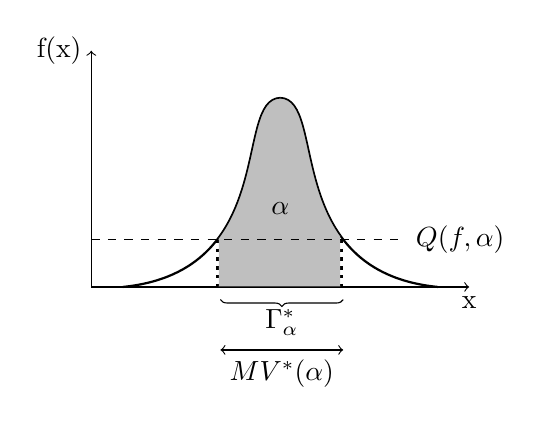
\begin{tikzpicture}[scale=2]

\draw[->](7.8,0)--(10.2,0) node[below]{x};
\draw[->](7.8,0)--(7.8,1.5) node[left]{f(x)}; 
\draw [thick] (8,0) ..controls +(1,0.1) and +(-0.3,-0.01).. (9,1.2);
\draw [thick] (9,1.2) ..controls +(0.3,-0.01) and +(-1,0.1).. (10,0);

\draw[dotted,very thick](8.60,0.3)--(8.60,0) node[right]{};
\draw[dotted,very thick](9.39,0.3)--(9.39,0) node[right]{};

%\draw (8,0.3)--(10,0.3)--(10,1.5)--(8,1.5)--(8,0.3); dessine 4 segments correspondant au 4 points

%hachurage :
\begin{scope} 
\clip (8.61,0)--(9.38,0)--(9.38,1.5)--(8.61,1.5)--(8.61,0) ; %tout ce qui est dans begin{scope} se limitera au rectangle

\path[draw,fill=lightgray] (8,0) ..controls +(1,0.1) and +(-0.3,-0.01).. (9,1.2)--
(9,1.2) ..controls +(0.3,-0.01) and +(-1,0.1).. (10,0)--
(8,0)--(10,0) --cycle;
\end{scope}

\draw[dashed](7.8,0.3)--(9.8,0.3) node[right]{$Q(f,\alpha)$};

%accolade :
\draw[decorate,decoration={brace}]
(9.4,-0.08)--(8.62,-0.08) node[below,pos=0.5] {$\Gamma_\alpha^*$};

\draw[<->]
(9.4,-0.4)--(8.62,-0.4) node[below,pos=0.5] {$MV^*(\alpha)$};



\draw (9,0.5) node[thick]{ $\alpha$} ;
%\draw (8.8,-0.8) node[thick]{Figure 1: MV curve} ;
\end{tikzpicture}
\caption{Mass-Volume at level $\alpha$}
\label{MVcurve}
\end{figure}


 % Practicaly, $\hat s$ will be of type $\sum_k \mathds{1}_{x\in \hat \Omega_{\alpha_k}^*}  $ where $(\alpha_k)$ is a subdivision of $[0,1[$.\\
The way of doing it consists in preliminarily estimating a collection of minimum volume sets related to target masses $0<\alpha_1<\ldots<\alpha_K<1$ forming a subdivision of $(0,1)$ based on training data so as to define $s=\sum_k \mathds{1}_{x\in \hat \Gamma_{\alpha_k}^*}$. The analysis is done under adequate assumptions (related to $\mathcal{G}$, the perimeter of the $\Gamma^*_{\alpha_k}$'s and the subdivision step in particular) and for an appropriate choice of $K=K_n$.
However, by construction, learning rate bounds are rather slow (of the order $n^{-1/4}$ namely) and cannot be established in the unbounded support situation.

But the four main drawbacks of this mass-volume curve criterion are the following.
\begin{itemize}
\item[\textbf{1)}] When used as a performance criterion, the Lebesgue measure of possibly very complex sets has to be computed.
\item[\textbf{2)}] When used as a performance criterion, there is no simple manner to compare MV-curves since the area under the curve is potentially infinite. %the pseudo-inverse $\alpha_s^{-1}(\alpha)$ may be hard to compute.
\item[\textbf{3)}] When used as a learning criterion (in the ERM paradigm), it produces level sets which are not necessarily nested, on which may be built inaccurate scoring function. 
\item[\textbf{4)}] When used as a learning criterion, the learning rates are rather slow (of the order $n^{-1/4}$ namely), and cannot be established in the unbounded support situation.
\end{itemize}



%%%%%%%%%%%%%  XXX to be removed if intro to long ?  %%%%%%%%%%%%%%%%%%%%%%
Figure \ref{algo-problem} illustrates the third drawback (mentioned above). In the $2$-d situation described here, given the training sample and the partition of the feature space depicted, the mass-volume criterion leads to consider the sequence of empirical minimum volume sets $A_1,\; A_1\cup A_2,\; A_1\cup A_3,\; A_1\cup A_2\cup A_3$ and thus the scoring function $s_1(x)=\mathbb{I}\{x\in A_1  \}+ \mathbb{I}\{x\in A_1\cup A_2  \} + \mathbb{I}\{x\in A_1\cup A_3  \}$, whereas the scoring function $s_2(x)=\mathbb{I}\{x\in A_1  \}+ \mathbb{I}\{x\in A_1\cup A_3  \}$ is clearly more accurate.
\begin{center}
\begin{figure}[h!]
\centering
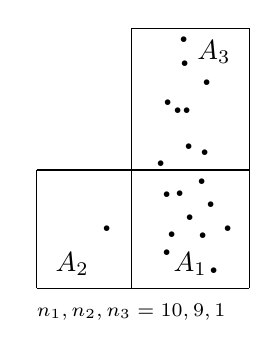
\begin{tikzpicture}[scale=1.5]

\draw[-](0.2,0)--(2,0) ;
\draw[-](0.2,0)--(0.2,1) ; 
\draw[-](1,0)--(1,2.2) ;
\draw[-](2,0)--(2,2.2) ;
\draw[-](0.2,1)--(2,1) ;
\draw[-](1,2.2)--(2,2.2) ;

\draw (0.8,0.5) node{\Huge .} ;
\draw (1.35,0.45) node{\Huge .} ;
\draw (1.3,0.79) node{\Huge .} ;
\draw (1.25,1.05) node{\Huge .} ;
\draw (1.31,1.57) node{\Huge .} ;
\draw (1.45,2.1) node{\Huge .} ;
\draw (1.47,1.5) node{\Huge .} ;
\draw (1.41,0.8) node{\Huge .} ;
\draw (1.49,1.2) node{\Huge .} ;
\draw (1.46,1.9) node{\Huge .} ;
\draw (1.4,1.5) node{\Huge .} ;

\draw (1.61,0.44) node{\Huge .} ;
\draw (1.68,0.71) node{\Huge .} ;
\draw (1.63,1.15) node{\Huge .} ;
\draw (1.64,1.74) node{\Huge .} ;
\draw (1.5,0.6) node{\Huge .} ;
\draw (1.7,0.15) node{\Huge .} ;
\draw (1.3,0.3) node{\Huge .} ;
\draw (1.82,0.5) node{\Huge .} ;
\draw (1.6,0.9) node{\Huge .} ;



\draw (1.5,0.2) node{$A_1$} ;
\draw (0.5,0.2) node{$A_2$} ;
\draw (1.7,2.) node{$A_3$} ;

\draw (1,-0.2) node{\scriptsize $n_1,n_2,n_3=10,9,1$} ;
\end{tikzpicture}
\caption{Unsuccessful mass-volume criterion optimization}
\parbox{13cm}{~\\ \footnotesize Sample of $n=20$ points in a $2$-d space, partitioned into three rectangles.  As $\alpha$ increases, the minimum volume sets $\hat \Gamma_{\alpha}$ are successively equal to $A_1$,~ $A_1 \cup A_2$,~ $A_1 \cup A_3$, and $A_1 \cup A_3 \cup A_2$, whereas, in the excess-mass approach, as $t$ decreases, the $\hat \Omega_{t}$'s are successively equal to $A_1$,~ $A_1 \cup A_3$,~ and $A_1 \cup A_3 \cup A_2$.
%$\hat \Omega_{10/20}=A_1$,~~ $\hat \Omega_{11/20}=A_1 \cup A_2$,~~ $\hat \Omega_{12/20}=A_1 \cup A_3$
}

\label{algo-problem}
\end{figure}
\end{center}
%%%%%%%%%%%%%%%%%%%%%%%%



In the following section, and as a contribution of this thesis, an alternative functional criterion is proposed, obtained by exchanging objective and constraint functions in \eqref{eq:MV}. The drawbacks of the mass-volume curve criterion are resolved excepting the first one, and it is shown that optimization of an empirical discretized version of this performance measure yields scoring rules with convergence rates of the order $\mathcal{O}_{\mathbb{P}}(1/\sqrt{n})$. In addition, the results can be extended to the situation where the support of the distribution $F$ is not compact. Also, when relaxing the assumption made in the mass-volume curve analysis that all level sets are included in our minimization class $\mathcal{A}$, a control of the model bias is established. Last but not least, we derive (non-statistical) theoretical properties verified by this criterion, which corroborate its role as a metric on preorders/level sets summarized in scoring functions.


\subsection{The Excess-Mass criterion}
\label{resume:em-curve}
The contribution summarized here has been published in~\cite{AISTAT15}.
We propose an alternative performance criterion which relies on the notion of \textit{excess mass} and \textit{density contour clusters}, as introduced in the seminal contribution \cite{Polonik95}. The main idea is to consider a Lagrangian formulation of a constrained minimization problem, obtained by exchanging constraint and objective in \eqref{eq:MV}: for $t>0$,
\begin{equation}
\label{solomeg}
\max_{\Omega~ \text{borelian}}  \left\{ \mathbb{P}(\mb X \in \Omega) - t \leb(\Omega) \right\}.
\end{equation}
We denote by $\Omega^*_t$ any solution of this problem. This formulation offers certain computational and theoretical advantages both at the same time: when letting (a discretized version of) the Lagrangian multiplier $t$ increase from $0$ to infinity, one may easily obtain solutions of empirical counterparts of \eqref{solomeg} forming a \textit{nested} sequence of subsets of the feature space, avoiding thus deteriorating rate bounds by transforming the empirical solutions so as to force monotonicity.
%
%\subsubsection{Theoretical study}
The \textbf{optimal Excess-Mass curve} related to a given probability distribution $F$ is defined as the plot of the mapping $$t>0~~\mapsto~~ EM^*(t):=\max_{\Omega\text{ borelian} } \{ {\mathbb{P}} (\mb X\in \Omega)-t\leb(\Omega) \}.$$ 
Equipped with the notation above, we have: $EM^*(t)=\mathbb{P}(\mb X \in \Omega_t^*)-t \leb(\Omega_t^*)$ for all $t>0$.
Notice also that $EM^*(t) = 0$ for any $t>\|f\|_\infty:=\sup_{x\in \rset^d}\vert f(x)\vert$. 
%
The  \textbf{Excess-Mass curve} of $s\in\mathcal{S}$  w.r.t. the probability distribution $F$ of a random variable $\mb X$ is the plot of the mapping
\begin{equation}
\label{EM}
EM_s : t \in [0, \infty[ \mapsto \sup_{A \in \{(\Omega_{s,l})_{l>0}\}}\{ {\mathbb{P}}(\mb X \in A) - t \leb(A)\},
\end{equation}
where $\Omega_{s,t}=\{ x \in \rset^d, s(x) \ge t \}$ for all $t>0$.
One may also write $EM_s$ in terms of $\lambda_s$ and $\alpha_s$ defined in \eqref{eq:alpha_beta}, $EM_s(t)= \sup_{u>0}~ \alpha_s(u) -t \lambda_s(u) $. Finally, under assumption $\mathbf{A_1}$, we have $EM_s(t)=0$ for every $t> \|f\|_\infty$. 
%
\begin{center}
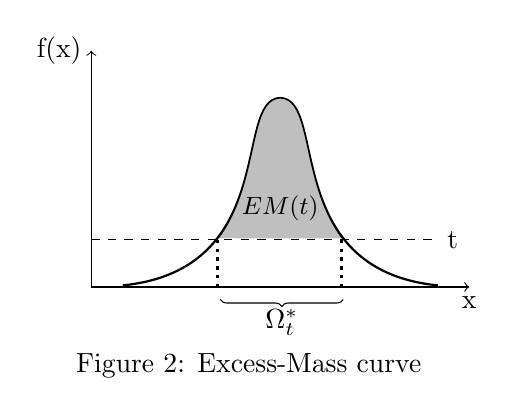
\begin{tikzpicture}[scale=2]
\draw[->](7.8,0)--(10.2,0) node[below]{x};
\draw[->](7.8,0)--(7.8,1.5) node[left]{f(x)}; 
\draw [thick] (8,0.01) ..controls +(1,0.1) and +(-0.3,-0.01).. (9,1.2);
\draw [thick] (9,1.2) ..controls +(0.3,-0.01) and +(-1,0.1).. (10,0.01);
\draw[dashed](7.8,0.3)--(10,0.3) node[right]{t};
\draw[dotted,very thick](8.60,0.3)--(8.60,0) node[right]{};
\draw[dotted,very thick](9.39,0.3)--(9.39,0) node[right]{};
%
%\draw (8,0.3)--(10,0.3)--(10,1.5)--(8,1.5)--(8,0.3); dessine 4 segments correspondant au 4 points
%
%hachurage :
\begin{scope} 
\clip (8,0.31)--(10,0.308)--(10,1.5)--(8,1.5)--(8,0.308) ; %tout ce qui est dans begin{scope} se limitera au rectangle (8,0.3)--(10,0.3)--(10,1.5)--(8,1.5)--(8,0.3)
\path[draw,fill=lightgray] (8,0) ..controls +(1,0.1) and +(-0.3,-0.01).. (9,1.2)--
(9,1.2) ..controls +(0.3,-0.01) and +(-1,0.1).. (10,0)--
(8,0.3)--(10,0.3) --cycle;
\end{scope}

%accolade :
\draw[decorate,decoration={brace}]
(9.4,-0.08)--(8.62,-0.08) node[below,pos=0.5] {$\Omega_t^*$};

\draw (9,0.5) node[]{\small $EM(t)$} ;
\draw (8.8,-0.5) node[thick]{Figure 2: Excess-Mass curve} ;
\end{tikzpicture}
\label{EMcurve}
\end{center}
%
\noindent
Maximizing $EM_s$ can be viewed as recovering a collection of subsets $(\Omega^*_t)_{t>0}$ with maximum mass when penalized by their volume in a linear fashion. An optimal scoring function is then any $s\in \S$  with the $\Omega^*_t$'s as level sets, for instance any scoring function of the form
\begin{align*}
%\label{score_cont}
s(x)=\int_{t=0}^{+\infty} \mathds{1}_{x\in \Omega^*_t}a(t)dt,\end{align*}
with $a(t)>0$ (observe that $s(x)=f(x)$ for $a \equiv 1$).
%
The mapping $EM_s$ is non increasing on $(0,+\infty)$, takes its values in $[0,1]$ and satisfies, $EM_s(t) \le EM^*(t)$ for all $t\geq 0$. 
In addition, for $t \ge 0$ and any $\epsilon > 0$, we have 
\begin{align*}
%\label{i}
\inf_{u>0} \epsilon \leb (\{ s >u\}\Delta_\epsilon \{f>t\}) ~\le~ EM^*(t)-EM_s(t) ~\le~ \|f\|_\infty \inf_{u>0} \leb (\{ s >u\}\Delta\{f>t\})
\end{align*}
with $\{ s >u\}\Delta_\epsilon \{f>t\} ~:=~~ \{f>t+\epsilon\} \setminus \{ s >u\} ~~~\bigsqcup~~~ \{ s >u\} \setminus \{f>t-\epsilon\}$. Thus the quantity $EM^*(t)-EM_s(t)$ measures how well level sets of $s$ can approximate those of the underlying density.
Under some reasonable conditions (see \cite{AISTAT15}, Prop.1), we also have 
for $\epsilon >0$, 
\begin{align*}
%\label{ii}
\sup_{t\in[\epsilon ,\|f\|_\infty]}|EM^*(t)-EM_s(t)| ~~\le~~  C \inf_{T  \in \mathcal{T}} \|f-T\circ s\|_\infty
\end{align*}
where the infimum is taken over the set $\mathcal{T}$ of all measurable increasing transforms $T : \mathbb{R}_+ \rightarrow \mathbb{R}_+$.
The previous inequalities reveal that $\|EM^* - EM_s\|_\infty$ can be interpreted as a pseudo distance either between the level sets of $s$ and those of the true density $f$, either between the preorders induced by $s$ and $f$. % `in the space of the scoring function', \ie~in the space where the element corresponding to a function $s$ is the class of every increasing transform of $s$ (or equivalently the class of every function which have the same level sets than $s$).


%\subsubsection{M-estimation}
%\label{sec:EM}
The concept of EM-curve provides a simple way to compare scoring functions but optimizing such a functional criterion is far from straightforward. As was proposed in \cite{CLEM13} for the MV criterion,
%Now that we have a way to attest the quality of a scoring function, a natural approach is to optimize an empirical version of it 
optimization is done over some representative class of scoring functions, hopefully rich enough to provide a good approximation (small model bias) while simple enough to control the convergence rate. Here we consider scoring functions of the form
\begin{align*}
%\label{score}
s_N(x):= \sum_{k=1}^N a_k \mathds{1}_{x \in \hat{\Omega}_{t_k} }~, ~~~\text{with ~~~} \hat{\Omega}_{t_k}  \in \mathcal{G}
\end{align*}
where $\mathcal{G}$ is a VC-class of subset of $\rset^d$.
We arbitrary take $a_k:= (t_k-t_{k+1})$ such that the $\hat{\Omega}_{t_k}$'s correspond exactly to $t_k$ level sets $\{s \ge t_k\}$. Then, maximizing the Excess-Mass functionnal criterion is done by sequentially resolving, for $k=1,\ldots,N$,
\begin{align*}
\hat \Omega_{t_k} \in \argmax_{\Omega \in \mathcal{G}} \frac{1}{n}\sum_{i=1}^n\mathds{1}_{X_i \in \Omega}~-~t_k \leb(\Omega).
\end{align*}
The $\hat \Omega_{t_k}$'s solution of these optimization problems can always be choosen in such a way they are nested (unlike the analogous optimization problem for the mass-volume criterion). In other words, an inclusion constraint can be added to the previous optimization problem, without affecting the quality of the solution picked up. It allows to avoid forcing the solutions to be nested, yielding stronger convergence rates.
In the mass-volume criterion M-estimation framework, assumptions were made stipulating that the support of the distribution is compact, and that the VC-class $\mathcal{G}$ contains the true density level sets. Here we relax these assumptions, the first one by chosing adaptive levels $t_k$, and the second one by deriving a bias study. 
In a nutshell, the levels are chosen as $t_{k+1} =\frac{t_1}{(1+\frac{1}{\sqrt n})^{k}} $ and
we assume that there exists a countable subcollection of $\mathcal{G}$, $F=\{F_i\}_{i \ge 1}$ say, forming a partition of $\mathcal{X}$ and such that $\sigma (F) \subset \mathcal{G}$. Then
the model bias is $\|f-f_{F}\|_{L^1}$, where $f_{F}(x) := \sum_{i \ge 1} \mathds{1}_{x \in F_i} \frac{1}{\leb(F_i)} \int_{F_i}f(y)dy~$ is the best approximation (for the $L_2$-norm) of $f$ by piecewise functions on $F$.
We obtain then a bound with high probability $1-\delta$,
\begin{align*}
\sup_{t \in ]0,t_1]}|EM^*(t)-EM_{s_N}(t)| ~\le~ \left[A+\sqrt{2\log(1/\delta)}\right]\frac{1}{\sqrt n} + \|f-f_{F}\|_{L^1}  + o_N(1), 
\end{align*}
with $A$ being an absolute constant, $t_1$ some initial parameter and $o_N(1)=1-EM^*(t_N)$. 
Recall incidentally that we are interested in minimizing $|EM^*(t)-EM_{s_N}(t)|$ for thresholds $t$ close to $0$, so that the value of $t_1$ is not important.
In addition, $s_N(x)$ converges to $s_\infty(x):=\sum_{k=1}^{\infty} (t_{k+1}-t_k)\mathds{1}_{\hat \Omega_{t_{k+1}}}$ as $N \rightarrow \infty$ and $s_\infty$ is such that, for all $\delta \in (0,1)$, we have with probability at least $1-\delta$,
\begin{align*}
\sup_{t \in ]0,t_1]}|EM^*(t)-EM_{s_\infty}(t)| \le \left[A+\sqrt{2\log(1/\delta)}\right]\frac{1}{\sqrt n} + \|f-f_{F}\|_{L^1}.
\end{align*}





\section{Evaluation of AD algorithms}
\label{resume:evaluation}
This is a summary of Chapter~\ref{chap:evaluation}, which is based on a workshop paper \citep{ICMLworkshop16} and a submitted work \citep{NIPS16evaluation}.


When sufficient labeled data are available, classical criteria based on \emph{Receiver Operating Characteristic} (ROC) or \emph{Precision-Recall} (PR) curves can be used to compare the performance of unsupervised anomaly detection algorithms. However, in many situations, few or no data are labeled. This calls for alternative criteria one can compute on non-labeled data.

While excess-mass and mass-volume curves quantities have originally been introduced to build scoring functions \emph{via}
Empirical Risk Minimization (ERM), the MV-curve has been used recently for the calibration of the One-Class SVM \citep{Thomas2015}.
When used to attest the quality of some scoring function, the volumes induced become unknown and must be estimated, which is challenging in large dimension if no prior knowledge on the form of these level sets is available.
%
Besides, there has been no work yet studying the accuracy of EM or MV curves as evaluation criteria.
%
Summarized in this section and as a contribution of this thesis, numerical performance scores based on EM and MV criteria (that do not require labels) are empirically shown to discriminate accurately (\wrt~ROC or PR based criteria) between algorithms.
%These criteria are based on existing Excess-Mass (EM) and Mass-Volume (MV) curves, which generally cannot be well estimated in large dimension.
A methodology based on feature sub-sampling and aggregating is also described and tested. This extends the use of these criteria to high-dimensional datasets and solves major drawbacks inherent to standard EM and MV curves.

Recall that the MV and EM curves of a scoring function $s$ can be written as
\noindent
\begin{align}
\label{intro:MV-def}
 MV_s(\alpha) &= \inf_{u \ge 0}~~ \leb(s \ge u) ~~\st~~\mathbb{P}(s(\mb X) \ge u) \ge \alpha\\
\label{intro:EM-def}
 EM_s(t) &= \sup_{u \ge 0}~~ \mathbb{P}(s(\mb X) \ge u) ~-~ t \leb(s \ge u)
\end{align}
for any $\alpha\in (0,1)$ and $t >0$.
%
The optimal curves are $MV^* = MV_f = MV_{T \circ f}$ and $EM^* = EM_f = EM_{T \circ f}$ for any increasing transform $T: \text{Im(f)} \to \mathbb{R}$
%
As curves cannot be trivially compared, consider the $L^1$-norm $\|.\|_{L^1(I)}$ with $I\subset \rset$ an interval. As $MV^*=MV_f$ is below $MV_s$ pointwise, $\argmin_s \| MV_s - MV^* \|_{L^1(I)} = \argmin \| MV_s \|_{L^1(I)} $. We thus define
$\crit^{MV}(s) = \| MV_s \|_{L^1(I^{MV})},$ which is equivalent to consider $\| MV_s - MV^* \|_{L^1(I^{MV})}$ as mentioned in the introduction. As we are interested in evaluating accuracy on large density level-sets, one natural interval $I^{MV}$ would be for instance $[0.9, 1]$. However, MV diverges in $1$ when the support is infinite, so that we arbitrarily take $I^{MV} = [0.9, 0.999].$
The smaller is $\crit^{MV}(s)$, the better is the scoring function $s$.
%
Similarly, we consider $\crit^{EM}(s) = \| EM_s \|_{L^1(I^{EM})}, $ this time with $I^{EM} = [0,EM^{-1}(0.9)],$ where $EM_s^{-1}(0.9) := \inf\{t\ge 0,~ EM_s(t) \le 0.9\}$, as $EM_s(0)$ is finite (equal to $1$). % We point out that such small values of $t$ correspond to large level-sets. Also in practice, we have observed that
% $EM_s^{-1}(0.9)$ (as well as $EM_f^{-1}(0.9)$) varies significantly depending on the dataset. Generally, for datasets in large dimension, it can be % $\widehat{EM}_s^{-1}(0.9)$ is
% very small (in the experiments, smallest values are of order $10^{-7}$) as it is of the same order of magnitude as the inverse of the total support volume.

As the distribution $F$ of the normal data is generally unknown, MV and EM curves must be estimated. Let $s\in \mathcal{S}$ and $\mb X_1,\; \ldots,\; \mb X_n$ be an i.i.d. sample with common distribution $F$ and set $\mathbb{P}_n(s \ge t)=\frac{1}{n}\sum_{i=1}^n\mathds{1}_{s(\mb X_i)\geq t}.$ The empirical MV and EM curves of $s$ are then simply defined as empirical version of \eqref{intro:MV-def} and \eqref{intro:EM-def}, 
\begin{align}
\label{MV-def-emp}
\widehat{MV}_s(\alpha) = \inf_{u \ge 0} \left\{ \leb(s \ge u) ~~\st~ \mathbb{P}_n(s \ge u) \ge \alpha \right\}
\end{align}
\begin{align}
\label{EM-def-emp}
\widehat{EM}_s(t) = \sup_{u \ge 0} \mathbb{P}_n(s \ge u) ~-~ t \leb(s \ge u)
%\lambda_s \circ \alpha_s^{-1}(\alpha),
\end{align}
%
%
Finally, we obtain the empirical EM and MV based performance criteria:
\begin{align}
\label{eq:standard_emp_EM}\widehat{\crit}^{EM}(s) &= \| \widehat{EM}_s \|_{L^1(I^{EM})}  &&I^{EM} = [0,\widehat{EM}^{-1}(0.9)],\\
\label{eq:standard_emp_MV}\widehat{\crit}^{MV}(s) &= \| \widehat{MV}_s \|_{L^1(I^{MV})}  &&I^{MV} = [0.9, 0.999].
\end{align}
%
% As the distribution $F$ is generally unknown, excess-mass curves must be estimated. Let $s\in \S$ and $\mb X_1,\; \ldots,\; \mb X_n$ be an i.i.d. sample with common distribution $F$ and set $$\widehat{\alpha}_s(t)=(1/n)\sum_{i=1}^n\mathds{1}_{s(X_i)\geq t}.$$ The empirical $EM$ curve of $s$ is then defined as $$\widehat{EM}_s(t)=\sup_{u>0}\{ \widehat{\alpha}_s(u)-t\lambda_s(u)\}.$$ In practice, just as with the mass-volume criterion (drawback \textbf{1}), it may be difficult to estimate the volume $\lambda_s(u)$ and Monte-Carlo approximation can naturally be used for this purpose.

% Note that in practice, the volume $\leb(s \ge u)$ is estimated using Monte-Carlo approximation, which only applies to small dimensions.
% %
% This is a major drawback for the use of excess-mass or mass-volume criteria in high dimensional framework, if no prior knowledge on the form of these level sets is available. Besides, there has been no work yet dealing with EM or MV curves as evaluation criteria, as they have originally been introduced to build scoring scoring function via ERM.
%
The methodology to scale the use of the EM and MV criteria to large dimensional data consists in sub-sampling training \emph{and} testing data along features, thanks to a parameter $d'$ controlling the number of features randomly chosen for computing the (EM or MV) score. Replacement is done after each draw of features $F_1,\ldots,F_{m}$. A partial score $\widehat \crit_k^{MV}$ (resp. $\widehat \crit_k^{EM}$) is computed for each draw $F_k$ using \eqref{eq:standard_emp_EM} (resp. \eqref{eq:standard_emp_MV}). The final performance criteria are obtained by averaging these partial criteria along the different draws of features. This methodology is described in Algorithm~\ref{algo:EMMV}.
%
\begin{algorithm}[!tbh]
\caption{~~High-dimensional EM/MV: evaluate AD algorithms on high-dimensional data}
\label{algo:EMMV}
\begin{algorithmic}
  \STATE \textbf{Inputs}: AD algorithm $\mathcal{A}$, data set $X = (x^j_i)_{1 \le i \le n, 1 \le j \le d }$, feature sub-sampling size $d'$, number of draws $m$.
  \FOR{$k=1,\ldots,m$}
    \STATE{randomly select a sub-group $F_k$ of $d'$ features}
    \STATE{compute the associated scoring function $\widehat s_{k} = \mathcal{A}\big((x^j_i)_{1 \le i \le n,~j \in F_k}\big)$}
    \STATE compute $\widehat{\crit}_k^{EM} = \| \widehat{EM}_{\widehat s_k} \|_{L^1(I^{EM})}$ using \eqref{eq:standard_emp_EM} or $\widehat{\crit}_k^{MV} = \| \widehat{MV}_{\widehat s_k} \|_{L^1(I^{MV})}$ using \eqref{eq:standard_emp_MV}
  \ENDFOR 
  \STATE \textbf{Return} performance criteria: $$\widehat{\crit}^{EM}_{high\_dim} (\mathcal{A})= \frac{1}{m} \sum_{k=1}^m\widehat \crit_k^{EM} \text{~~~~(idem for MV)}$$
\end{algorithmic}
\end{algorithm}

Low-dimensional and high-dimensional EM/MV are tested \wrt~three classical AD algorithms. A wide range on real labeled datasets are used in the benchmark.
Experiments show that when one algorithm has % \emph{clearly} (according to both EM and PR scores)
better performance than another on some fixed dataset, according to both ROC and PR AUCs, one can expect to recover it without using labels with an accuracy of $82\%$ in the novelty detection framework, and $77\%$ in the unsupervised framework.


\section{One-Class Random Forests}
\label{resume:ocrf}
This is a summary of Chapter~\ref{chap:ocrf}, which is based on submitted work \citep{OCRF16}.

Scoring functions built by optimizing EM or MV criteria usually not perform well. Indeed, optimization is done over some class of scoring functions \emph{hopefully rich enough to provide a good approximation while simple enough to control the convergence rate}. This compromise is to optimistic in practice, specially in high dimension. In addition, if criterion optimization is useful when no intuition is available on the underlying problem, this is not the case in anomaly detection. We usually do not try to minimize ROC curves to have a good classifier, and a doctor usually does not health people by trying to optimize tensiometer or stethoscope measurements. 
%
To derive guaranties of theoretical nature (namely to attest the relevance of the algorithm in terms of \eg~ROC or EM/MV criteria), optimizing these evaluation criteria is often an efficient way. 
But this does not remains true in terms of empirical performance. % There is example of methods 
% having few or no theoretical guaranties %, this is not the case anymore. %mecanic does'nt repair motors by trying to minimize the sensors
%
In this section, we propose to build scoring functions using Random Forests (RFs). RFs \citep{Breiman2001} are an intuitive way of performing classification and regression. More formally, we adapt RFs to the one-class classification framework by introducing one-class splitting criteria.

Standard RFs are estimators that fit a number of decision tree
classifiers on different random sub-samples of the dataset.
Each tree is built recursively, according to a splitting criterion based on
some impurity measure of a node. The prediction is done by an average over each tree prediction. In classification the averaging is based on a majority vote.
Few attempts to transfer the idea of RFs to one-class
classification have already been made \citep{Desir12, Liu2008, Shi2012}
%, Clemencon2014}. On ne cite pas clemencon2014 car leur algorythm treeRank n'est pas des RFs (base estimator = non-symetric ranking trees) (en fait unsupervisedTreeRank c'est juste une modif triviale de TreeRank en considerant des volumes)
%
No algorithm structurally extends (without second class sampling and without alternative base estimators) RFs to one-class classification.

We introduce precisely such a methodology. It builds on a natural adaptation of two-class % Gini improvement proxy, yielding a one-class Gini-based criterion specially designed for
splitting criteria to the one-class setting, as well as an adaptation of the two-class majority vote.
In addition, it turns out that the one-class model promoted here corresponds to the asymptotic behavior of an adaptive (with respect to the tree growing process) outliers generating methodology.


Let us summarize our One-Class Random Forest algorithm, based on generic RFs \citep{Breiman2001}. It has $7$ parameters:
$max\_samples$, $max\_features\_tree$, $max\_features\_node$, $\gamma$, $max\_depth$, $n\_trees$, $s_k$.

Each tree is classically grown on a random subset of both the input samples and the input features \citep{Ho1998, Panov2007}.
This random subset is a sub-sample of size $max\_samples$, with $max\_features\_tree$ variables chosen at random without replacement (replacement is only done after the tree is grown). The tree is built by minimizing 
a one-class version of the Gini criterion \citep{Gini1912}, obtained by replacing empirical quantities related to the second class by theoretical ones induced by an uniform distribution, increasingly weighted during the tree building process in order to avoid highly unbalanced classes, as the nodes more and more tend to have small volume while containing as much (normal) observations as possible.
%
Minimization of this criterion is done until the maximal depth $max\_depth$ is achieved.
% define a large number of geometric features and search over a random selection
% of these for the best split at each node
In addition, this is done as introduced in \citep{Amit1997}, defining a large number $max\_features\_node$ of geometric features and searching over a random selection of these for the best split at each node.
%
The forest is composed of a number $n\_trees$ of trees. The predicted score of a point $x$ is given by $s_k(x)$, which is either the stepwise density estimate (induced by the forest) around $x$, the local density of a typical cell containing $x$ or the averaged depth of $x$ among the forest.




\section{Extreme Values Analysis through STDF estimation}
\label{resume:stdf}
This section is a summary of Chapter~\ref{colt}, which is based on previous work published in \cite{COLT15}.

We have seen that scoring functions are built
by approaching density level sets/minimum volume sets of the underlying `normal' density. As mentioned previously, for an anomaly detection purpose, we are interested in being accurate on level sets corresponding to high quantiles, namely with level $t$ close to $0$ -- equivalently being accurate on minimum volume sets with large mass constraint $\alpha$.  
%
In the univariate case, suppose we want to consider the $(1-p)^{th}$ quantile of the distribution $F$ of a random variable $X$, for a given exceedance probability $p$, that is $x_p = \inf\{x \in \mathbb{R},~ \mathbb{P}(X > x) \le p\}$. For moderate values of $p$, a natural empirical estimate is $x_{p,n} = \inf\{x \in \mathbb{R},~ 1/n \sum_{i=1}^n \mathds{1}_{X_i > x}\le p\}$.
However,  if $p$ is very small, the finite  sample $X_1,\ldots, X_n$  contains insufficient information and $x_{p,n}$ becomes irrelevant.
%
This problem transfers in the multivariate case to learning density level sets with very low level, or equivalently scoring functions inducing such level sets.
%
Extreme value theory specially adresses such issues, in the one-dimensional as well as in the multi-dimensional setup.



\paragraph{Preliminaries.}
Extreme Value Theory (\textsc{EVT}) develops models for learning the unusual rather than the usual. These models are widely used in fields involving risk management like finance, insurance, telecommunication or environmental sciences. One major application of \textsc{EVT} is to provide a reasonable assessment of the probability of occurrence of rare events. 

To illustrate this point, suppose we want to manage the risk of a portfolio containing $d$ different assets, $\mb X = (X_1,\ldots,X_d)$. A fairly general purpose is then to evaluate the probability of events of the kind $\{X_1 \ge x_1 \text{ or }  \dotsc \text{ or } X_d\ge x_d \}$, for large multivariate thresholds $\mb x=(x_1,\ldots,x_d)$. Under not too stringent conditions on the regularity of $\mb X$'s  distribution, \textsc{EVT} shows that for large enough thresholds, 
\[
\P\{X_1 \ge x_1 \text{ or }  \dotsc \text{ or }
X_d\ge x_d \} \simeq 
l(p_1,\ldots,p_d), 
\]  
where $l$ is the  \emph{stable tail dependence function} (STDF) and the $p_j$'s  are the marginal exceedance probabilities, $p_j = \P(X_j\ge x_j)$. The functional $l$ characterizes the \emph{dependence} among extremes. The \emph{joint} distribution (over large thresholds) can thus be recovered from the knowledge of the marginal distributions  together with the \textsc{stdf} $l$. In practice, $l$ can be learned from `moderately extreme' data, typically the $k$ `largest' ones among a sample of size $n$, with $k\ll n$.

Recovering the $p_j$'s can be done following a well paved way: in the univariate case, \textsc{EVT} essentially consists in modeling the distribution of the maxima (\emph{resp.} the upper tail) as a generalized extreme value distribution, namely an element of the Gumbel, Fréchet or Weibull parametric families (\emph{resp.} by a generalized Pareto distribution).

In contrast, in the multivariate case, there is no finite-dimensional parametrization of the dependence structure. 
The latter being characterized by the \textsc{stdf}, estimating this functional is one of the main issues in multivariate \textsc{EVT}. Asymptotic properties of the empirical \textsc{stdf} have been widely studied, see \cite{Huangphd}, \cite{Drees98}, \cite{Embrechts2000} and \cite{dHF06} for the bivariate case, and \cite{Qi97}, \cite{Einmahl2012} for the general multivariate case under smoothness assumptions.

However, no bounds exist on the finite sample error. The contribution summarized in the next section and published in \cite{COLT15} derives such non-asymptotic bounds. Our results do not require any assumption other than the existence of the \textsc{stdf}. 




\paragraph{Learning the dependence structure of rare events.}
Classical VC inequalities aim at bounding the deviation of empirical from theoretical quantities on relatively simple classes of sets, called VC classes. These classes typically cover the support of the underlying distribution.  However, when dealing with rare events, it is of great interest to have such bounds on a class of sets which only covers a small probability region and thus contains (very) few observations. This yields sharper bounds, since only differences  between very small quantities are involved. The starting point of this analysis is the following VC-inequality stated below.
\begin{theorem}
\label{thm-princ} 
Let $\mathbf{X}_1,\ldots,\mathbf{X}_n$ be \iid~realizations of a \rv~$\mathbf{X}$, a VC-class $\mathcal{A}$ with VC-dimension $V_{\mathcal{A}}$. %and shattering coefficient (or growth function) $S_{\mathcal{A}}(n)$.
% Let us consider a sample $X_1,...,X_n$ of $n$ \iid~realizations of a
% \rv~$X$ in $\mathbb{R}^d$, and $\mathcal{A}$ a VC-class of sets of
% $\mathbb{R}^d$. 
Consider the class union $\mathbb{A} = \cup_{A \in \mathcal{A}} A$,
 and let  
$p = \mathbb{P}(\mathbf{X} \in \mathbb{A})$. Then there is an absolute constant $C$ such that for all $0<\delta<1$, with probability at least $1-\delta$,
\begin{align*}
\sup_{A \in \mathcal{A}} \left| \mathbb{P} \big[\mathbf{X} \in A\big] - \frac{1}{n} \sum_{i=1}^n \mathds{1}_{\mathbf{X}_i \in A}  \right| ~~\le~~ C \bigg[ \sqrt{p}\sqrt{\frac{V_{\mathcal{A}}}{n} \log{\frac{1}{\delta}}} + \frac{1}{n} \log{\frac{1}{\delta}} \bigg]~.
\end{align*}
\end{theorem}


The main idea is as follows. The empirical estimator of the {\sc stdf} is based on the empirical measure of `extreme' regions, which  are hit only with  low probability. It is thus enough to bound  maximal deviations on such low probability regions. 
 The key consists in choosing an adaptive VC class, which only covers the latter regions, and on the other hand, to derive VC-type inequalities that incorporate $p$, the probability of hitting the class at all. The bound we obtain on the finite sample error is then:

\begin{theorem}
\label{thm:l}
%Let $k(n)$ a sequence of  
Let $T$ be a positive number such that $T \ge \frac{7}{2}(\frac{\log d}{k} + 1)$, and $\delta$ such that $\delta \ge e^{-k}$. Then there is an absolute constant $C$ such that for each $n >0$, with probability at least $1-\delta$:
\begin{align*}
\sup_{0 \le \mathbf{x} \le T} \left| l_n(\mathbf{x}) - l(\mathbf{x})
\right| ~\le~ Cd\sqrt{\frac{T}{k}\log\frac{d+3}{\delta}} ~+~ \sup_{0
  \le \mathbf{x} \le 2T}\left|\frac{n}{k} \tilde
  F(\frac{k}{n}\mathbf{x})- % {\red \frac{n}{k}l ( \frac{k}{n}
  % \mathbf{x}) =
l(\mb x)\right|
\end{align*}
where $l$ is the \stdf, and by definition $l(\mathbf{x})= \lim_{t \to 0} t^{-1} \tilde F (t\mathbf{x}) $ such that the second term in the bound is a bias term.
\end{theorem}


In this section, we have introduced and studied, in a non-parametric setting, a particular functional characterizing the extreme dependence structure.
%
One other convenient (nonparametric) characterization of  extreme dependence in the framework of multivariate EVT is the \textit{angular measure}, which provides direct information about the probable `directions' of extremes, that is, the relative contribution of each feature/coordinate of the `largest' observations.
%
In many applications, it is more convenient to work with the angular measure itself. The latter gives more direct information on the dependence structure and is able to reflect structural simplifying properties (\eg~sparsity as detailed below) which would not appear in extreme value copulas or in the STDF which are integrated version of the angular measure.
However, non-parametric modeling of the angular measure faces major difficulties, stemming from its potentially complex structure, especially in a high dimensional setting.
Further, from a theoretical point of view, non-parametric estimation of the angular measure has only been studied in the two dimensional case, in \cite{Einmahl2001} and \cite{Einmahl2009}, in an asymptotic framework. As another contribution of this thesis, the section below summarizes a novel methodology (presented in \cite{AISTAT15}, \cite{NIPSWORKSHOP15} and a long version under review \cite{ARXIV16}) aiming at exhibiting a sparsity pattern within the dependence structure of extremes.



\section{Sparse Representation of Multivariate Extremes}
\label{resume:sec:JMVA}
This section is a summary of Chapter~\ref{jmva}, which is based on previous work published in \cite{AISTAT15} and on work \cite{ARXIV16} under review.
\subsection{Context: multivariate extreme values in large dimension}
\label{context}

Parametric or semi-parametric estimation of the structure of multivariate extremes is relatively well documented in the statistical literature, see  \emph{e.g.} \cite{coles1991modeling,fougeres2009models,cooley2010pairwise,sabourinNaveau2012} and the references therein. However, restrictive structural assumptions have to be made, stipulating \emph{e.g.} that only some pre-definite subgroups of components may be concomittantly extremes, or, on the contrary, that all of them must be. In addition, their practical use is restricted to moderate dimensional problems (say, $d\le 10$), otherwise simplifying modeling choices are needed, as \emph{e.g.} in \cite{stephenson2009high}). Finally, uncertainty assessment concerning the output of these models is made under the hypothesis that the training set is `asymptotic', in the sense that one assumes that, above a fixed high threshold, the data are exactly distributed according to the limit distribution of extremes. In other words, the modeling error is ignored. 

Non-parametric estimation of the angular measure has only been treated in the two dimensional case, in \cite{Einmahl2001} and \cite{Einmahl2009}, in an asymptotic framework. Here we extend the nonasymptotic study on {\sc stdf} estimation (previous section) to the angular measure of extremes, restricted to a well-chosen class of sets, corresponding to lower-dimensional regions of the space. The objective is to learn a representation of the angular measure, rough enough to control the variance in high dimension and accurate enough to gain information about the `probable directions' of extremes, both at the same time. This yields a --first-- non-parametric estimate of the angular measure in any dimension, restricted to a class of subcones, %XXX Fig.
with a non asymptotic bound on the error. 
Note incidentally that this method can also be used as a preprocessing stage, for dimensionality reduction purpose, before proceeding with a parametric or semi-parametric estimation which could benefit from the structural information issued in the first step. Such applications are beyond the scope of this thesis.

The framework we develop is non-parametric and lies at the intersection of support estimation, density estimation and dimensionality reduction: it consists in learning the support of a distribution (from training data), that can be decomposed into subcones, hopefully each of low dimension and to which some mass is assigned, defining empirical versions of probability measures of specific extreme regions. 
It produces a scoring function defined and specially accurate on extreme regions, which can thus be exploited to detect anomalies among extremes.
Due to its moderate complexity --of order $d n \log n$-- this algorithm is suitable for the treatment of real word large-scale learning problems, and experimental results reveal a significantly increased performance on extreme regions compared with standard anomaly detection approaches. 



In a wide range of situations, one may expect the occurrence of two phenomena:

\textbf{1-} Only a `small' number of groups of components may be concomitantly extreme, so that only a `small' number of hyper-cubes (those corresponding to these subsets of indexes precisely) have non zero mass (`small' is relative to the total number of groups $2^d$).

\textbf{2-} Each of these groups contains a limited number of coordinates (compared to the original dimensionality), so that the corresponding hyper-cubes with non zero mass have small dimension compared to $d$.

The main purpose of this work is to introduce a data-driven methodology for identifying such faces, so as to reduce the
dimensionality of the problem and thus to learn a sparse representation  of extreme behaviors. 
In case hypothesis \textbf{2-} is not fulfilled, such a sparse  `profile' can still be learned, but loses the low dimensional property of its supporting hyper-cubes.
One major issue is that real data generally do not concentrate on sub-spaces of zero Lebesgue measure. This is circumvented by setting to zero any coordinate less than a threshold $\epsilon>0$, so that the corresponding `angle' is assigned to a lower-dimensional face. 

More formally, Figures \ref{fig:3Dcones} and \ref{2Dcones} represent the transformed input space, resulting from classical standardization of the margins. After this non-linear transform, the representation of extreme data is linear and learned by estimating the mass on the sub-cones
\begin{align*}
 \mathcal{C}_\alpha = \{\mb v \ge 0,~\|\mb v\|_\infty \ge 1,~ v_j > 0 ~\text{ for } j \in \alpha,~ v_j = 0 ~\text{ for } j \notin \alpha \},
\end{align*}
or more precisely, the mass of the angular measure $\Phi$ on the corresponding sub-spheres
\begin{align*}
\Omega_{\alpha}  = \{\mb x \in S_{\infty}^{d-1} :  x_i > 0 \text{ for } i\in\alpha~,~  x_i = 0 \text{ for } i\notin \alpha   \} 
 = S_{\infty}^{d-1}\cap {\mathcal{C}}_\alpha,
\end{align*}
represented in Figure~\ref{fig:3Dcones}.

\noindent
\begin{minipage}{0.5\linewidth}
\centering
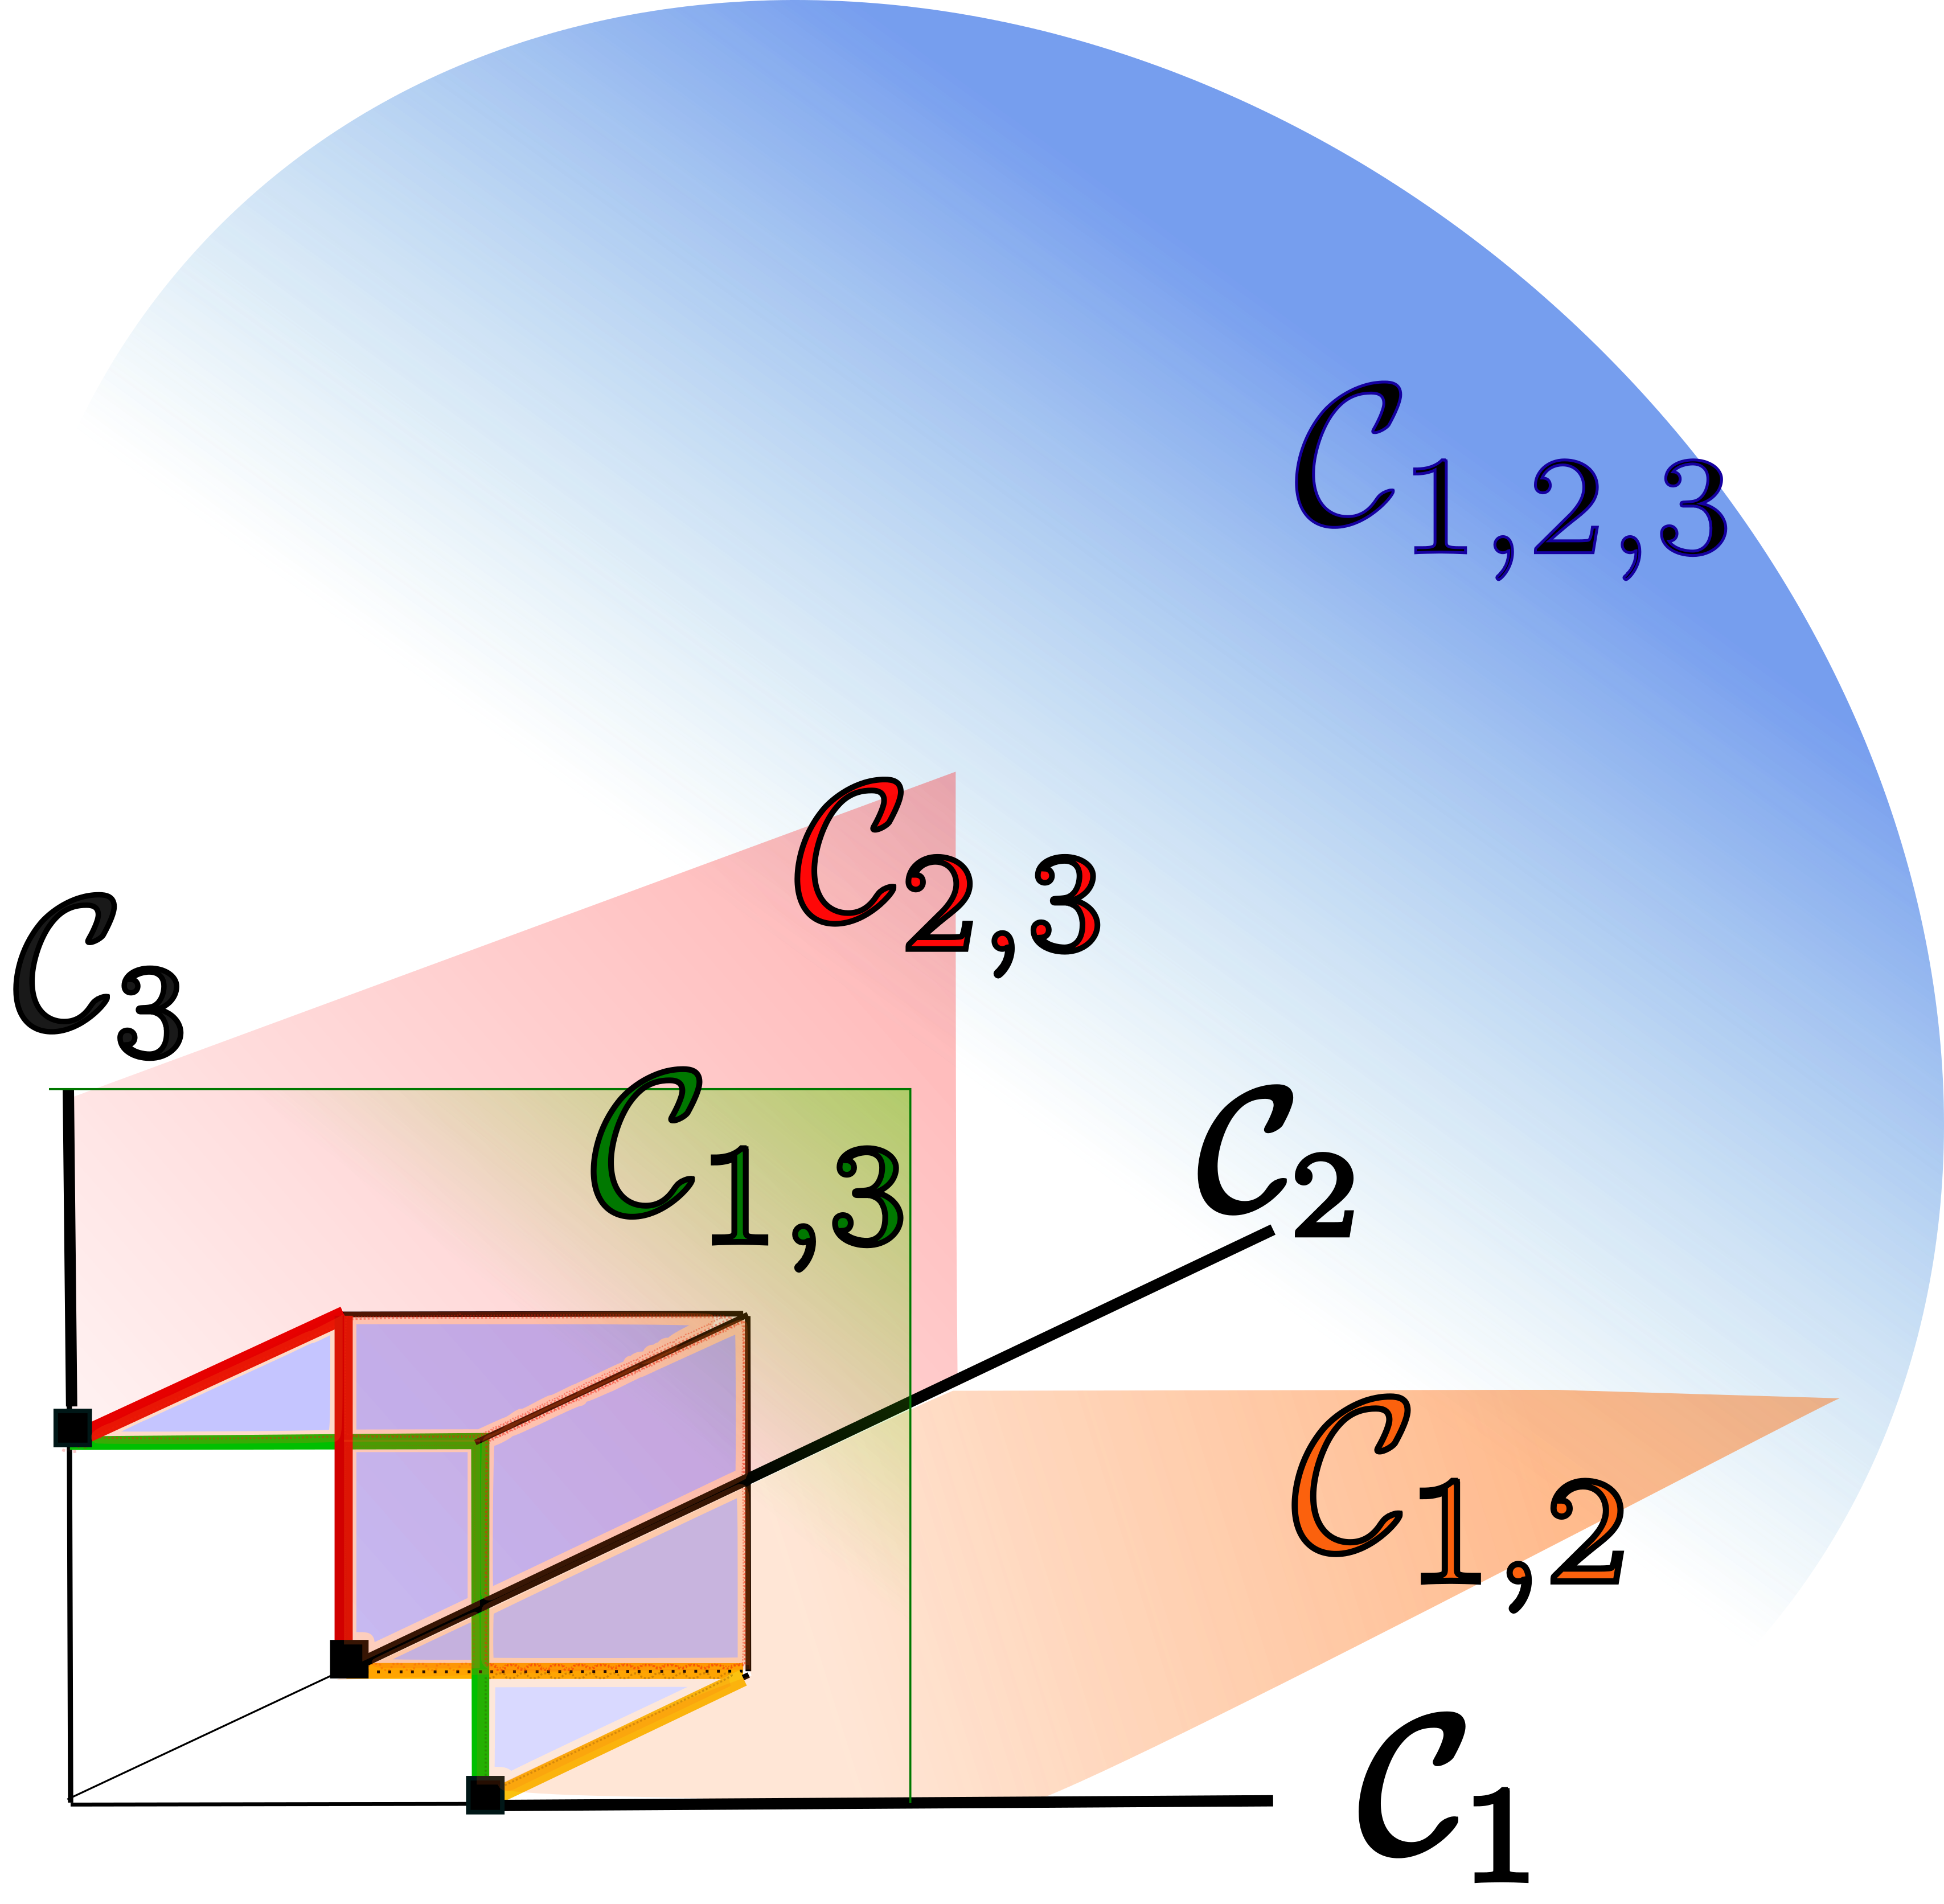
\includegraphics[scale=0.2]{fig_source/cone}
\captionof{figure}{Truncated cones in 3D}
\label{fig:3Dcones}
\end{minipage}\hfill
\begin{minipage}{0.5\linewidth}
\centering
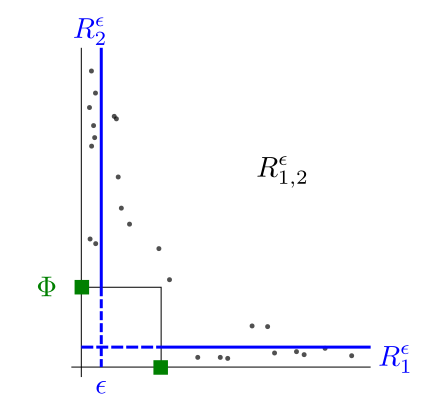
\includegraphics[width=0.64\linewidth]{fig_source/representation2D}
\captionof{figure}{Truncated $\epsilon$-cones in 2D}
\label{2Dcones}
\end{minipage}


This is done using $\epsilon$-thickened sub-cones $\cone_\alpha^\epsilon$, corresponding to $\epsilon$-thickened sub-spheres $\Omega_\alpha^\epsilon$, as shown in Figure~\ref{2Dcones} in the two-dimensional case.
We thus obtain an estimate $\widehat{\mathcal{M}}$ of the representation
$$\mathcal{M} = \{ \Phi(\Omega_{\alpha}):\; \emptyset \neq \alpha\subset\{1,\; \ldots,\; d \}\}.$$
Theoretically, recovering the $(2^{d}-1)$-dimensional unknown
vector $\mathcal{M}$ amounts to roughly approximating the support of $\Phi$ using the partition
$\{\Omega_\alpha, \alpha\subset\{1,\ldots,d\}, \alpha\neq \emptyset\}$, that is, determine which $\Omega_\alpha$'s have
nonzero mass (and evaluating the mass $\Phi(\Omega_\alpha)$), or equivalently, which $\Phi_\alpha$'s are nonzero. This support estimation is potentially
sparse (if a small number of $\Omega_\alpha$ have non-zero mass, \ie~Phenomenon~\textbf{1-}) and
potentially low-dimensional (if the dimensions of the sub-spheres $\Omega_\alpha$ with non-zero mass are low, \ie~Phenomenon~\textbf{2-}).

% Second, investigate how the angular measure $\Phi$ spreads its mass on the
% $\Omega_{\alpha}$'s, the theorical quantity $\Phi(\Omega_{\alpha})$ indicating to which extent extreme observations may occur in the `direction' $\alpha$ for $\emptyset \neq \alpha \subset \{1,\; \ldots,\; d \}$. 

% These two goals are achieved using empirical versions of
% the angular measure, evaluated on the $\epsilon$-thickened sub-spheres $\Omega_\alpha^\epsilon$.


\subsection{Algorithm and Application to Anomaly Detection}

As explained above, the proposed algorithm, DAMEX for Detecting Anomalies with Extremes, learns a (possibly sparse and low-dimensional) representation of the angular measure. This representation is rough enough to control the variance in high dimension and accurate enough to gain information about the `probable directions' of extremes. From a theoretical perspective, it yields a --first-- non-parametric estimate of the angular measure in any dimension, restricted to a class of sub-spheres. %, with a non asymptotic bound on the error. 
We believe that our method can also be used as a preprocessing stage, for dimensionality reduction purpose, before proceeding with a parametric or semi-parametric
estimation of the angular measure which could benefit from the structural information issued in the first step.  Such applications are beyond the scope of this work and will be the subject of further research. 

%The representation output by DAMEX may be exploited to detect anomalies among extremes.
EVT has been intensively used in anomaly detection in the one-dimensional
situation, see for instance \cite{Roberts99}, \cite{Roberts2000},
\cite{Clifton2011}, \cite{Clifton2008}, \cite{Lee2008}.
% Anomaly detection then relies on tail analysis of the variable of interest and naturally involves EVT.
In the multivariate setup, however, there is --to the best of our
knowledge--  no anomaly detection method
relying on \textit{multivariate} EVT. Until now, the multidimensional case has only been  tackled by means of extreme value statistics
based on univariate EVT. The major reason is 
the difficulty to scale up existing multivariate EVT models
with the dimensionality. In the present work we bridge the gap between the practice of anomaly detection and multivariate EVT by proposing a method which is
able to learn a sparse `normal profile' of multivariate extremes and,
as such, may be implemented to improve the accuracy of any usual anomaly detection algorithm.




Let $\mb X_1,.\ldots,\mb X_n$ \iid random variables in $\mathbb{R}^d$ with joint
(\emph{resp.} marginal) distribution $\mb F$ (\emph{resp.} $F_j$, $j =
1,\ldots,d$). Marginal standardization is a natural first step when
studying the dependence structure in a multivariate setting. The
choice of standard Pareto margins $V^j$ (with $\mathbb{P}(V^j > x ) =
1/x$, $x>0$) is convenient, and justified by multivariate extreme value theory (see Chapter~\ref{back:EVT}). One classical way to standardize is the
probability integral transform, $T : X_i \mapsto V_i = ( (1- F_j
(X_i^j))^{-1})_{1\leq j\leq d}$, $i = 1,\ldots,n$. 
%
Since the marginal distributions $F_j$ are unknown, we use their
empirical counterpart $\hat F_j$, where $\hat F_j (x) =
(1/n) \sum_{i=1}^n \mathds{1}_{X_i^j\le x}$. 
Denote by $\hat T$ the rank transformation
thus obtained and by $\hat V_i = \hat T(X_i)$ the corresponding rank-transformed
observations. 

Now, for a given subset of features $\alpha \subset \{1,...,d\}$
the goal is to measure the
% `correlation' within each
%  at extreme levels, that is
likelihood to observe a large $\mathbf{\hat V}$ such that $\hat V^j$ is `large' for all
$j\in\alpha$, while the other $\hat V^j$'s ($j \notin \alpha$) are `small'.
That is, estimating $\Phi(\Omega_\alpha)$.
% Formally, one may %has to 
% associate to each such $\alpha$ a coefficient
% %$\mu_n^\alpha$ 
% reflecting the degree of dependence between the
% features $\alpha$ at extreme levels. %By definition of asymptotic dependence, 

In relation to Section~\ref{context}, the appropriate way to
give a meaning to `large' (\emph{resp.} `small') among extremes is in
`radial' and `directional' terms, that is, $\| \mathbf{\hat V}\|>r$ (for some
high radial threshold $r$), and $\hat V^j/\|\mathbf{\hat V}\| >\epsilon$
(\emph{resp.} $ \le \epsilon$) for some small directional tolerance
parameter 
$\epsilon>0$.
Introduce the truncated $\epsilon$-cones (see Fig.~\ref{2Dcones}):
%\begin{align*}
$ ~\mathcal{C}_\alpha^\epsilon~=~\big\{\mb v \ge 0,~\|\mb v\|_\infty \ge 1,~ v_i > \epsilon \|\mb v\|_\infty ~\text{ for } i
 \in \alpha, ~~v_i \le \epsilon\|\mb v\|_\infty ~\text{ for } i \notin \alpha~ \big\},$
%\end{align*}
which defines a
partition of $\mathbb{R}_+^{d}\setminus [0,1]^d$ for each fixed $\epsilon\ge 0$.
This leads to  estimates %$\mu_n^{\alpha, \epsilon}$  of the form
\begin{align}
\label{mu_n}
\Phi_n^{\alpha, \epsilon} = (n/k) \mathbb{\hat P}_n \left (  (n/k) \mathcal{C}_\alpha^\epsilon \right), 
\end{align}
\noindent
where $\mathbb{\hat P}_n(.)=(1/n)\sum_{i=1}^n\delta_{\hat{\mb V}_i}(.)$ is the empirical probability distribution of the rank-transformed data and $k =
k(n) \to \infty$ s.t. $k = o(n)$ as $n \to
\infty$. %  Indeed we are to select the extreme observations to
% study asymptotic dependence, from where the $\frac{n}{k}
% \mathcal{C}_\alpha^\epsilon$ (
The ratio $n/k$ plays the role of a large radial
threshold $r$. 
This estimator is justified by the result from multivariate EVT, $r \mathbb{P}(\mb V \in r A) \to \Phi(A)$ as $r \to \infty$ (see Chapter~\ref{back:EVT}).
% From our standardization choice, counting points in
% $(n/k)\,\mathcal{C}_{\alpha}^{\epsilon}$ boils down to
% selecting, for each feature $j\le d$,   the `$k$ largest values' $X_i^j$
% over the $n$ observations, whence the normalizing factor $\frac{n}{k}$.
%Here and hereafter, $k =
%k(n) >0$ is such that $k \to \infty$ and $k = o(n)$ as $n 
%\infty$.
%

This heuristic yields the following algorithm~\ref{DAMEX-algo}.
The complexity is in $O( dn\log n + dn) = O(dn\log n)$, where the first term on the left-hand-side comes from  computing the $\hat F_j(X_i^j)$ (Step 1) by sorting  the data
(\emph{e.g.} merge sort). The second one comes from Step 2. 

% \begin{center}
% \fbox{
% \begin{minipage}{0.95\linewidth}
\begin{algorithm}[!tbh]
\caption{DAMEX}
\label{DAMEX-algo}
{\bf Input:} parameters $\epsilon>0$,~~ $k = k(n)$,~~ $\Phi_{\min}\geq 0$.
\begin{enumerate}
\item Standardize \emph{via} marginal rank-transformation: $\hat V_i := \hat T(X_i) =  \big (1/(1- \hat F_j (X_i^j))\big)_{j=1,\ldots,d}$~. %\\where $\hat F_j (X_i^l) = \frac{1}{n}(rank(X_i^l)-1)$.
% \item Let $k = n^{2/3}$, $\epsilon = \frac{1}{ k}$ 
\item Assign to each $\hat V_i$ the cone $\mathcal{C}_\alpha^\epsilon$
  it belongs to.  
\item Compute  $\Phi_n^{\alpha, \epsilon}$ the estimate of the $\alpha$-mass of $\Phi$ from (\ref{mu_n}).\\
 $\rightarrow$ yields: (small number of) cones with non-zero mass.
\item (Optional) Set to $0$ the $\Phi_n^{\alpha,\epsilon}$ below some small
  threshold $\Phi_{\min}\ge 0$ to eliminate cones with negligible mass
   
\end{enumerate}
{\bf Output:} (sparse) representation of the dependence
  structure %$(\mu_n^{\alpha,\epsilon})_{\alpha\subset\{1,\ldots, d\}, \mu_n^{\alpha,\epsilon}>\mu_{\min}}$.
 \begin{align*}
\widehat{\mathcal{M}}(\alpha) := (\Phi_n^{\alpha,\epsilon})_{\alpha\subset\{1,\ldots, d\}, \Phi_n^{\alpha,\epsilon}>\Phi_{\min}}
 \end{align*}

\end{algorithm}
% \end{minipage}
% }
% \end{center}

This algorithm can directly be applied to anomaly detection.
The underlying assumption is that an
observation is potentially abnormal if its `direction' (after a standardization of each marginal) is special
regarding the other extreme observations. In other words, if it
does not belong to the (sparse) support of
extremes.
The degree of `abnormality' of a new observation $\mb x$ such that
$\hat T(\mb x) \in \mathcal{C}_\alpha^\epsilon$ % an observation $X_i$
should be related both to $\Phi_n^{\alpha, \epsilon}$ and the uniform
norm $\|\hat T(\mb x)\|_\infty$ (angular and radial
components). As a matter of fact, in the transformed space - namely the
space of the $\hat V_i$'s - the asymptotic mass decreases as the
inverse of the norm.
Consider the  `\textit{directional tail region}' induced by $\mb x \in \mathcal{C}_\alpha^\epsilon$, 
$A_{\mb x} =  \{\mb y  :
T(\mb y) \in \mathcal{C}_\alpha^\epsilon\,,\;\|T(\mb y)\|_\infty \ge \|
T(\mb x)\|_\infty\}.$
 Then, if  $\|T(\mb x)\|_\infty$ is large enough, it can be shown that 
$  \mathbb{P}( \mb X \in A_{\mb x} ) \simeq  \|\hat T(\mb x) \|_\infty^{-1} \Phi_n^{\alpha,\epsilon} $.
We then set the scoring function $$s_n(\mb x):= (1/\|\hat T(\mb x)\|_\infty) \sum_{\alpha }\Phi_n^{\alpha, \epsilon} \mathds{1}_{\hat T(\mb x) \in \mathcal{C}_\alpha^\epsilon},$$
which is thus an empirical version of
$\mathbb{P}(\mb X\in A_{\mb x})$: the smaller $s_n(\mb x)$, the more abnormal the point $\mb x$ should be considered.


\subsection{Theoretical grounds}

From the work on the \stdf~estimation summarized in the previous Section~\ref{resume:stdf}, in particular from Theorem~\ref{thm-princ} and from the ideas used to prove Theorem~\ref{thm:l}, we are able to derive some theoretical guaranties for the approach described above. %  where non-asymptotic
% bounds related to the statistical performance of a non-parametric
% estimator of the \emph{stable tail dependence function} (STDF), another 
% functional measure of the dependence structure of extremes,  are
% established.  
% However, even in the case of a sparse angular measure, the support of
% the STDF would not be so, since the latter functional is  an
% integrated version of the former. Also, 
% in many applications, it is more convenient to work with % an alternative (distributional)
%  the {angular measure}. Indeed, it provides direct information about the probable `directions' of extremes. % , that is, the relative contribution
% % of each components of the `largest' observations  (where `large' may be 
% % understood \emph{e.g.} in the sense of the infinity norm on the input
% % space). We emphasize again that estimating these `probable relative contributions' is a major concern in many fields
% % involving  the management of risks from multiple sources, \emph{e.g.}\,portfolio monitoring, insurance,
% % environmental risk management and anomaly detection. 
% To the best of our knowledge, non-parametric estimation of the angular
% measure has only been treated in the two dimensional case, in
% \cite{Einmahl2001} and \cite{Einmahl2009}, in an asymptotic
% framework.

Under non-restrictive assumptions standard in EVT (existence of the angular measure and continuous marginal c.d.f.), we obtain a non-asymptotic bound of the form
\begin{align*}
\sup_{\emptyset \neq \alpha \subset \{1,\; \ldots,\; d \}}~ |\widehat{\mathcal{M}}(\alpha)- \mathcal{M}(\alpha)|
~\le~  C d \left( \sqrt{ \frac{1}{\epsilon k}\log\frac{d}{\delta}} + M d\epsilon \right) + \text{bias}(\epsilon, k, n),
\end{align*}
with probability greater than $1-\delta$, where $k = k(n) \to \infty$ with $k(n) = o(n)$ can be interpreted as the number of data considered as extreme. 
The bias term goes to zero as $n \to \infty$, for any fixed $\epsilon$.




\subsection{Empirical grounds}
 The main purpose of Algorithm~\ref{DAMEX-algo} is to deal with extreme data. We evaluate its performance on such region and compare it with a standard anomaly detection algorithm, the Isolation Forest (iForest) algorithm, see Section~\ref{sec:impl} below, which we chose in view of its established high performances (\cite{Liu2008}) and its ability to handle large dimensional data. 
The two algorithms are trained and tested on the same datasets, the test set being restricted to some extreme region.
Five reference real-word datasets in anomaly detection are considered. The experiments are performed in a semi-supervised framework (the training set consists of normal data). In a  non-supervised framework (training set including abnormal data), the improvements brought by the use of DAMEX are less significant, but the precision score is still increased when the recall is high (high rate of true positives), inducing more vertical ROC curves near the origin.
DAMEX significantly improves the performance (both in term of precision and of ROC curves) in extreme regions for each dataset.

XXX: comparaison avec LOF, OCSVM and EllipticEnvelop when possible?\\
XXX: study combination DAMEX with other classical AD?

\section{Scikit-learn contributions}
\label{sec:impl}

As an other contribution of this thesis, two classical anomaly detection algorithms, $IsolationForest$ and $LocalOutlierFactor$ have been implemented and merged on scikit-learn. These algorithms are presented in the Background Part, Section~\ref{sec:AD_sklearn}. % on Anomaly Detection in Scikit-Learn. 

Scikit-learn, see \cite{sklearn2011}, is an open-source library which provides well-established machine learning methods.
It is a Python module, the latter language being very popular for scientific computing, thanks to its high-level interactive nature. Python is enjoying this recent years a strong expansion both in academic and industrial settings. Scikit-learn takes advantage of this favourable backdrop and extends this general-purpose programming language with machine learning operation: % it not only provides implementations of many established algorithms, both supervised and unsupervised % (while keeping an easy-to-use interface tightly integrated with the Python language)
% , but
it provides a composition mechanism (through a \emph{Pipeline} object) to combine estimators, preprocessing tools and model selection methods in such a way the user can easily construct complex ad-hoc algorithms.
%
The development is done on \emph{Github}\footnote{https://github.com/scikit-learn}, a Git repository hosting service which facilitates collaboration, as coding is done in strong interaction with other developpers. Because of the large number of developers, emphasis is put on keeping the project maintainable, \eg~by avoiding dupplicating code at the price of a reasonable loss of computational perforance.%up to pay (reasonably) in computational performance. 


This contribution was supervised by Alexandre Gramfort and was funded by the Paris Saclay Center for Data Science. It also includes work for the scikit-learn maintenance like resolving issues and reviewing other contributors' pull requests.

XXX: add contribution with A.Muller


\section{Conclusion and Scientific Output}
The contributions of this thesis can be summarized as follows. 

First, it proposes (Section~\ref{resume:em-curve}) an adequate performance criterion, in order to compare possible candidate scoring function and to pick one eventually. 
The corresponding publication is \cite{AISTAT15}:
\begin{itemize}
\item On Anomaly Ranking and Excess-Mass Curves. (AISTAT 2015).\\
Authors: Goix, Sabourin, and Clémençon. 
\end{itemize}

However, the use of the Excess-Mass curve (just as Mass-Volume curve) to measure the quality of a scoring function $s_n$ involves the computation of the Lebesgue measure  $\leb(s_n \ge u)$, which is a major drawback for its use in high dimensional framework. Besides, these two criteria
have originally been introduced to build scoring functions \emph{via}
Empirical Risk Minimization (ERM), and no study has been made on their use to evaluate scoring functions as ROC or PR criteria do.
% This is a major drawback for its use in high dimensional framework, if no prior knowledge on the form of these level sets is available. 

As a second contribution, we show (empirically) that EM or MV based criteria are able to discriminate accurately (\wrt~ROC or PR based criteria) between scoring functions in law dimension. Besides, we propose a methodology based on feature sub-sampling and aggregating to scale the use of EM or MV to higher dimensions.
The corresponding publications are \cite{ICMLworkshop16} and \cite{NIPS16evaluation}:
\begin{itemize}
\item How to Evaluate the Quality of Unsupervised Anomaly Detection Algorithms? (ICML 2016, Workshop on Anomaly Detection). Co-winner of the Best Paper Award, sponsored by Google.\\
Author: Goix. 
\item How to Evaluate the Quality of Unsupervised Anomaly Detection Algorithms? (submitted to NIPS 2016).\\ Authors: Goix and Thomas. 
\end{itemize}

%However, to measure with this criterion the quality of a scoring function $s_n$, volume of level sets of $s_n$ have to be compute which is a considerable drawback for its use in high dimensional framework, if no prior knowledge on the form of these level sets is available.

The third contribution of this thesis is to develop an efficient way of building accurate scoring functions. This is done by generalizing random forests to one-class classification. The corresponding publication is 
\begin{itemize}
\item One-Class Splitting Criteria for Random Forests with Application to Anomaly Detection. (Submitted to NIPS 2016).\\
Authors: Goix, Brault, Drougard and Chiapino.
\end{itemize}


As a fourth contribution, we bring advances in multivariate EVT by providing non-asymptotic bounds for the estimation of the STDF, a functional characterizing the extreme dependence structure (Section~\ref{resume:stdf}). The corresponding publication is \cite{COLT15}:
\begin{itemize}
\item Learning the dependence structure of rare events: a non-asymptotic study. (COLT 2015).\\
Authors: Goix, Sabourin, and Clémençon.
\end{itemize}

The fifth contribution is to design a statistical method that produces a (possibly sparse) representation of the dependence structure of extremes, while deriving non-asymptotic bounds to assess the accuracy of the estimation procedure (Section~\ref{resume:sec:JMVA}).
%
This contribution also includes a multivariate EVT-based algorithm which returns a scoring functions defined in extremes region. This directly applies to anomaly detection as an abnormality score.
The corresponding publications are \cite{AISTAT16}, \cite{NIPSWORKSHOP15} and \cite{ARXIV16}:
%
\begin{itemize}
\item Sparse Representation of Multivariate Extremes with Applications to Anomaly Ranking. (AISTAT 2016 and NIPS 2015 Workshop on Nonparametric Methods for Large Scale Representation Learning).\\
Authors: Goix, Sabourin, and Clémençon.
\item Sparse Representation of Multivariate Extremes with Applications to Anomaly Detection. (Under review for Journal of Multivariate Analysis).\\
Authors: Goix, Sabourin, and Clémençon.
\end{itemize}


As a last contribution (of incremental nature), two classical anomaly detection algorithms have been implemented and merged on scikit-learn. They are used in this dissertation for empirical comparison to attest the relevance of the forementionned approaches.
The pull requests of these two contributions are available here:
\begin{itemize}
\item https://github.com/scikit-learn/scikit-learn/pull/4163  (Isolation Forest)
\item https://github.com/scikit-learn/scikit-learn/pull/5279 (LOF)
\end{itemize}


\paragraph{Context of this work}
This thesis was carried out in the STA (Statistiques et Applications) team of the Signal and Image Processing (TSI) department at Telecom ParisTech. The contributions presented in this thesis were supported by Ecole Normale Supérieure de Cachan via a `contrat doctoral pour normalien' and by the industrial chair `Machine Learning for Big Data' from Telecom ParisTech. The scikit-learn contributions have been supported by the Paris Saclay Center for Data Science regarding the collaboration with Alexandre Gramfort, and by the forementioned machine learning chair as regards the collaboration at New York University with Andreas Müller.

\paragraph{Outline of the thesis}
This dissertation is organized as follows. 
\begin{itemize}
\item Part~\ref{part:background} gathers the background work relevant to this thesis.
Chapter~\ref{back:AD_scikit} reviews classical anomaly detection algorithms through the scikit-learn library and presents implementative contributions of this thesis; Chapter~\ref{chap:back_concentration} presents general results on measure concentration inequalities; and Chapter~\ref{back:EVT} provides a concise background on Extreme Value Theory.

\item Part~\ref{part:struct} deals with unsupervised anomaly detection criteria.
Chapter~\ref{aistat:chap} presents the details on anomaly ranking and excess-mass curve, as summarized above Section~\ref{resume:scoring}. Chapter~\ref{chap:evaluation} deals with the evaluation of anomaly detection algorithms, as summarized above Section~\ref{resume:scoring}. Chapter~\ref{resume:evaluation}.

\item Part~\ref{part:ocrf} is about one-class random forests: Chapter~\ref{chap:ocrf} presents the details % on one class splitting criteria 
  summarized above Section~\ref{resume:ocrf}.

\item Part~\ref{part:vect} focuses on EVT-based methods for anomaly detection. Chapter~\ref{colt} deals with the stable tail dependence function as summarized above in Section~\ref{resume:stdf}. Chapter~\ref{jmva} describes how scoring functions can be build using EVT, as previously summarized in Section~\ref{resume:sec:JMVA}.
\end{itemize}
